
%
% ---- Chapter layout ----
%
% 1) Introduction - 
% 2) 
% ------------------------



\chapter{Biogenic Isoprene emissions in Australia} % Chapter title
\label{BioIsop}
  
%----------------------------------------------------------------------------------------
% Section 1 -- INTRO 
%----------------------------------------------------------------------------------------
\section{Introduction}  
\label{BioIsop:intro}  
  
  
  
  % isoprene and Australia
  Biogenic volatile organic compounds (BVOC) affect the oxidative capacity of the atmosphere and are largely driven by and sensitive to what type of vegetation is in the area \parencite{Kefauver2014}.
  In the troposphere, BVOC emissions affect the hydroxyl radical (OH) cycling, ozone (O$_3$) and secondary organic aerosol (SOA) production, and methane longevity.
  Australian forests are strong emitters of isoprene, the primary BVOC emitted globally \parencite{Guenther2006,Messina2016}. % and monoterpenes.
  However; emissions are poorly understood due to poor measurement coverage.
  The lack of measurements makes it difficult to estimate the subsequent atmospheric processes.% such as ozone and secondary organic aerosol (SOA) formation.
  Isoprene has a large impact on the oxidative properties of the atmosphere, as it reacts quickly with the OH radical.
  
  Emission models used to derive these an estimate of isoprene fluxes are based understanding of different plant species (phenotypes) in varying conditions, however these are seldom well understood within Australian forests.
  The chemistry involved is complex and still suffers from relatively large uncertainties in both measurement and chemistry mechanisms.
  Isoprene emissions may be overestimated in Australia since they are based on measurements taken from a few heavily emitting young eucalyptus trees which are not representative \parencite{Winters2009, FortemsCheiney2012,}.
  Emissions estimates can improve boundary conditions for atmospheric chemistry models without requiring expensive measurement campaigns over the large data sparse continent of Australia.
  %%BVOC emissions are rising globally, and improving estimates for Australia is a priority since they affect such important processes in the atmosphere.
  %\textcite{Kefauver2014} reviews remote sensing of BVOC emissions, examining the last 20 years of data and analysis of the satellite products.
  \textcite{Guenther2012} Estimated global biogenic isoprene emissions at roughly 535\tgpyr, while \textcite{Sindelarova2014} estimated around 411\tgpyr.
  %Guenther used MEGAN, \textcite{Sindelarova2014} estimated around 594\tgpyr using MEGAN with MACC, showing isoprene as 69.2\% of the total BVOC emissions, with monoterpenes at 10.9\tgpyr (10.9\%).
  
  In this chapter the we describe and use a technique using satellite measurements of HCHO to calculate surface isoprene emissions.
  HCHO is the dominant product of most BVOCs and is measured by satellites via remote sensing techniques.
  In situ isoprene concentration measurements are costly and sparse within Australia, while satellite HCHO data are plentiful and freely available, making this technique very attractive.
  Such techniques have informed isoprene emission inventories in North America \parencite{Abbot2003,Palmer2003,Palmer2006,Millet2006,Millet2008}, South America \parencite{Barkley2013}, Europe \parencite{Dufour2009,Curci2010}, Africa \parencite{Marais2012}, Asia \parencite{Fu2007,Stavrakou2014}, India \parencite{Surl2018}, and even globally \parencite{Shim2005,FortemsCheiney2012,Bauwens2016}.
  In this thesis the OMHCHO dataset from the OMI instrument (see Section \ref{Model:omhcho}) is used as the basis for HCHO amounts.
  
  \subsection{Aims}
    
    In Chapter \ref{Model}, the OMI HCHO total columns are recalculated using an updated estimate of HCHO profiles from GEOS-Chem v10.01 .
    These estimates are compared to available datasets of isoprene or HCHO (SPS1, SPS2, MUMBA, Wollongong FTIR) in Section \ref{BioIsop:results:measurements} %, Daintree) 
    Sensitivity satellite AMF calculation is examined and quantified for some scenarios.
    In this chapter we outline why current isoprene emissions estimates are inadequate and how they can be improved.
    We discuss literature which shows how the estimates may be too high, and describe how emissions may be calculated using satellite datasets.
    Section \ref{BioIsop:method} lays out how new isoprene emissions are estimated, with results examined in Section \ref{BioIsop:results}. 
    Uncertainties for each step along the way are quantified in Section \ref{BioIsop:uncertainty}.
    In Section \ref{BioIsop:conclusions} we examine how these changes in emissions would affect ozone concentrations in Australia, along with some other chemical processes.
    
    
    %% AIMs paragraph
    Recent work suggests that modelled emissions may be overestimated in Australia \parencite{Emmerson2016}.
    %, while emissions of monoterpenes (C$_{10}$H$_{16}$, two units of isoprene) appear to be underestimated . 
    %This could lead to the unique scenario of neither emission type dominating VOC chemistry over the forests.
    This work tries to improve the understanding of isoprene emissions over the whole of Australia, clarifying the spatial distribution of bias and how these biases impact modelled chemistry.
    We estimate isoprene emissions in Australia using top-down estimates based on OMI HCHO measurements and modelled yields.
    This a postiori top-down estimate is used to determine if model fit against sparse available ground-based measurements can be improved.
    GEOS-Chem model output is examined before and after updating isoprene emissions which are used as inputs.
    Wellness of fit between in situ (at Wollongong) HCHO, satellite (OMI), and modelled (GEOS-Chem) HCHO is determined with and without updated emissions estimates.
    
  \subsection{Existing emissions estimates}
    
    
    % Overestimates from models
    The Model of Emissions of Gases and Aerosols from Nature (MEGAN) is one of the most popular emissions inventories for biogenic isoprene.
    Along with other models which rely on measured plant emission rates, it is poorly calibrated for Australian conditions.
    Emissions of isoprene (C$_5$H$_8$) appear to be overestimated in some regions within Australia \parencite{Sindelarova2014,Stavrakou2014,Emmerson2016}.
    A lack of measurements of isoprene emission rates in Australia, along with missing soil moisture parameterisation are the most likely culprits TODO: cite.
    \textcite{Sindelarova2014} showed how the isoprene emissions could be as much as halved by accounting for lower soil moisture.
    \textcite{Stavrakou2015} saw isoprene emissions overestimated by a factor of 2-3 in January.
    \textcite{Emmerson2016} discuss the suitability of MEGAN's isoprene and monoterpene emission factors over southeast Australia, and suggest isoprene emissions are estimated 2-6 times too high.
    They also show that no blanket increase or decrease in emission factors is appropriate for the entire southeast of Australia.
    Additionally, emissions of monoterpenes (C$_{10}$H$_{16}$, two units of isoprene) appear to be underestimated \parencite{Emmerson2016}.
    %This could lead to the unique scenario of neither emission type dominating VOC chemistry over the forests.
    
    Recently \textcite{Bauwens2016} estimated isoprene emissions with a top-down technique using the IMAGESv2 global CTM.
    They calculate emissions which create the closest match between model and satellite vertical columns, and compare these a postiori data with their a priori (satellite data) and independent data sets.
    They examine global emissions seen by three models and a top-down inversion.
    For Australia they found emissions ranging from 26-94\tgcpyr.
    In this thesis we prioritise the analysis of a top-down emissions estimate compared against MEGAN, along with flow on effect of changed emissions on modelled ozone levels.
  
  \subsection{Top-down isoprene emissions estimates}
    \label{BioIsop:intro:top_down_estimates}
    
    % Brief isoprene to hcho description
    In the remote troposphere HCHO production is dominated by methane oxidation, while in the continental boundary layer production is largely due to non-methane VOCs (NMVOCs) \parencite{Abbot2003, Kefauver2014}.
    This leads to a causal relationship between enhanced HCHO concentrations and NMVOC emissions.
    In the continental boundary layer, HCHO enhancement is generally driven by short lived ($<1$~hr) precursors (most importantly isoprene).
    HCHO itself has a lifetime of a few hours \parencite{Kefauver2014}.
    Isoprene is emitted and enters the atmosphere in the gas phase, where it begins a complex series of reactions.
    Formaldehyde is produced with high yield in many reactions beginning with isoprene oxidation, discussed in more detail in Section \ref{LR:VOCs:IsopCascade}.
    
    % Lead in to satellite inversion
    Top-down estimates look at how much of a chemical is in the atmosphere and try to work out how much of its major precursors were emitted.
    This generally takes advantage of longer lived products which may reach a measurable equilibrium in the atmosphere.
    For isoprene this is done by looking at atmospheric HCHO enhancement, which can be largely attributed to isoprene emissions once transport and other factors are accounted for.
    %Even anthropogenic HCHO source estimates, which are accurate at the global scale, can be improved using satellite data to improve regional estimates by up to 25-40\% \parencite{Stavrakou2015}. 
    %Their study used the RETRO 2000 database for anthropogenic emission a prioris except for Asia in 2008 where REASv2 was used. 
    Since 1997, when GOME measurements were first used to measure HCHO over Asia \parencite{Thomas1998}, satellites have been used to provided a total column measurement of HCHO, allowing isoprene emissions estimates by proxy \parencite{Palmer2001,Bauwens2016}.
    Using satellite information to improve biogenic emissions is pinpointed as a valuable use of satellite derived datasets \parencite{Streets2013}.
    In this work we use NASA's OMHCHO product, using measurements from OMI on board the AURA satellite (see Section \ref{Model:omhcho}).
    
    There are two top-down isoprene emission estimation techniques, Bayesian and linear, which are discussed briefly here.
    Both the linear and Bayesian techniques assume that modelled chemistry is accurate and only try to correct precursor emissions, which may be a problem if the chemistry is uncertain.
    Uncertainties in the techniques are discussed in Section \ref{BioIsop:uncertainty:eomi}.
    
    %    Top-down emission estimation is an in-depth process, and a couple of examples are provided here.
    %    \textcite{Marais2014} compare OMI based isoprene emission estimates against relaxed eddy accumulation measurements from African field campaigns in order to improve MEGAN emission factors in the region.
    %    \textcite{Dufour2009} use HCHO from SCIAMACHY, and examine Europe using CHIMERE as the chemical model, showing that satellite measurements can reduce source emission uncertainty by a factor of two, where emissions are relatively large.
    %    There are two main methods of estimating isoprene emissions using satellite measurements of child products, here I describe them and briefly compare the pros and cons of each.
    %    
    
    \subsubsection{Bayesian}
    
      % Top down emissions estimation methods:
      Bayesian inversion corrects biased biogenic isoprene emissions by optimising emission parameters in order to reduce the differences between measured and modelled HCHO.
      Inversions can be set up to account for effects from transport and allow source attribution \parencite{FortemsCheiney2012}.
      
      In general a model (the forward model) is used to determine the relationship between HCHO ($y$) and the state variable \emph{x}, which represents isoprene and other variable parameters of interest:
      \begin{equation}
        \label{BioIsop:intro:top_down_estimates:eqn_bayesian}
        y=\mathbf{Kx} + b + \epsilon
      \end{equation}
      where $\epsilon$ are the (assumed) independent errors in measurements.
      \emph{K} is the Jacobian matrix determined from the forward model representing the sensitivity of $y$ to the state variable \emph{x}.
      Essentially the \emph{K} matrix is the modelled estimation of how $y$ responds to each of the driving parameters represented by elements of \emph{x}
      This \emph{K} matrix is used in conjunction with error covariance in \emph{x} to determine the most likely (maximum a postiori) solution to \emph{x}, given what we know about $y$. % ($\hat{x}$).
      
      For example this method is used by \textcite{Shim2005} who optimise GEOS-Chem isoprene emissions in areas with high HCHO concentrations to improve comparison against GOME HCHO observations. % They looking at areas with high signal to noise ratio (higher HCHO concentrations).
      They show that the original model underestimates isoprene emissions and HCHO concentrations by 14-46\%, with the corrected VOC emissions reducing model biases to 3-25\%.
      The Bayesian inversion is also used in \textcite{Curci2010}, where a regional CTM (CHIMERE) simulates HCHO (this is the forward model), which is compared against OMI observed HCHO and shown to be regionally biased.
      %The CHIMERE model is used to derive yields of HCHO from the various local VOCs and these are then used in estimating local emissions.
      The model is run initially with emissions of BVOCs and reactive anthropogenic VOCs turned off in order to work out the background ($b$) values of these compounds.
      \textcite{Curci2010} uses CHIMERE as the forward model to determine the relationship between HCHO and \emph{x}, which in this case is isoprene and reactive anthropogenic VOCs, then they calculate the most likely values for \emph{x} given known measured HCHO and modelled \emph{K}.
      
      
      An advantage of the Bayesian method is that it can account for pyrogenic and anthropogenic emissions rather than filtering them out.
      Biases may still arise due to errors in modelled emission estimation \parencite{Curci2010}.
      The Bayesian method is computationally expensive due to the requirement that model runs take place using many permutations of changed inputs.
      In this work we do not use the Bayesian method due to the heavy computational costs involved.
      
        
    
    \subsubsection{Linear}
      \label{BioIsop:intro:top_down_linear}
      
      This technique is the simplest, and is performed in this thesis.
      Using vertical columns of biogenic HCHO one can infer the local (grid space) isoprene emissions using effective molar formaldehyde yield (in other continents around 2-3, or 1 in low NO$_x$ conditions) \parencite{Palmer2003,Marais2012,Bauwens2016}.
      If one assumes fast HCHO yield, so that the effect of transport is minimal, and that HCHO and isoprene are at steady states, then one may calculate local yield from a CTM.
      %This yield is derived from both HCHO and isoprene, such as was used by \textcite{Millet2006} who produced a molar HCHO yield of 2.3 in north eastern USA.
      
      By assuming a simple linear steady-state relationship between HCHO and its precursors \parencite{Palmer2003, Palmer2006, Millet2006}, one may calculate isoprene emissions using measured HCHO.
      The calculation requires reaction rates and yields from isoprene to HCHO, which can be determined most readily using chemical modelling.
      The methodology for calculating isoprene emissions from HCHO is laid out in \textcite{Palmer2003}, and takes into account the expected lifetime and reaction rates of the precursor VOCs and HCHO.
      In their work isoprene emissions fluxes were derived using the Global Ozone Monitoring Experiment (GOME) satellite instrument.
      Palmer's method improved biogenic isoprene emissions estimates (compared with in situ measurements) over two available inventories: the U.S. EPA Biogenic Emissions Inventory System and the Global Emissions Inventory Activity. %(BEIS2)(GEIA).
      An outline of how this method is applied in this thesis is given in Section \ref{BioIsop:method:outline}.
      
      % Pros and cons:
      This technique assumes fast HCHO yield and no precursor transport, which is unrealistic in several scenarios; e.g. high winds can lead to transported precursors, or low NO$_x$ concentrations can slow down HCHO yield.
      Filtering out potentially problematic scenarios can limit the utility of this technique depending on environmental factors.
      As we are estimating biogenic emissions of isoprene, we must also filter out areas where HCHO may be coming from anthropogenic or pyrogenic sources.
      On the plus side, the simple nature of the inversion requires very little computational power after acquiring satellite and model datasets, even over large amounts of gridded data.
      
    
\section{Methods}
  \label{BioIsop:method}
  
  
  % First isoprene inversion work
  We broadly follow the method of \textcite{Palmer2001} to create an emissions estimate of isoprene over Australia.
  In this work yield is calculated from the modelled slope between isoprene emissions and HCHO tropospheric columns within each gridbox over Australia, as performed in \textcite{Palmer2003}, using modelled values between 1300-1400 LT which is around the overpass time of the OMI.
  This modelled yield is then used in conjunction with the recalculated OMI measurements in order to estimate isoprene emissions.
  To calculate this yield we use a reduced major axis (RMA) regression between modelled average values of the total columns and isoprene emission rates, an example is shown in Figure \ref{BioIsop:method:fig_RMA_example} shows the modelled regression between emissions and tropospheric columns for January, 2005. Also shown is the time series for these two quantities averaged over Australia, and the squared correlation coefficient along with a sample from four grid squares.
  
  %Plot from GC_tests.py -> Examine_Model_Slope()
  \mypic{/Figures/OMI_link/GC/E_isop_vs_hcho_200501.png}{%
    Top left: RMA slope between modelled tropospheric column HCHO ($\Omega_{GC}$) and isoprene emissions ($E_{GC}$) using midday (13:00-14:00~LT) values over for January 2005, per grid square at \lowhr horizontal resolution.
    Top right: Australia-wide average of midday emissions and tropospheric columns.
    Bottom left: Squared RMA correlation coefficient for regression in top left. Coloured dots correspond to colour of regressions shown in bottom right panel.
    Bottom right: Sample of correlations from four grid squares.}
  {\label{BioIsop:method:fig_RMA_example}}
  
  
  
  \subsection{Outline}
    \label{BioIsop:method:outline}
    % Method Briefly outlined here
    This section provides an overview of the steps involved in creating a top-down emissions estimate. %, from reading satellite data and model output to the creation of isoprene emissions estimates.
    This process is summarised in Figure \ref{BioIsop:method:fig_Flow_Making_Isop}.
    \begin{enumerate}
      \item 
        Corrected vertical columns ($\Omega$; saved in OMHCHORP dataset) are calculated (see Section \ref{Model:omiRecalc}) using level two OMI HCHO satellite data (see Section \ref{Model:omhcho}), along with GEOS-Chem model runs (see Section \ref{Model:GC:simulations}) at \highhr horizontal resolution.
      \item 
        Level three satellite data are used to make anthropogenic, fire, and smoke influence masks (see Section \ref{Model:filter}).
        These are applied to remove $\Omega$ which may be influenced by pyrogenic or anthropogenic sources. 
      % Mini list for masking taken from here
      \item 
        GEOS-Chem modelled biogenic emissions of isoprene ($E_{GC}$) along with total biogenic columns of HCHO ($\Omega_{GC}$), both averaged over \lowhr horizontally and 13:00-14:00~LT temporally, are used to calculate a reduced major axis linear regression slope ($\Omega_{GC}=S E_{GC} + \Omega_{GC;0}$).
        Calculation of this modelled slope is explained in Section \ref{BioIsop:method:slope}.
      %\item For each of the corrected vertical columns (VCC$_{OMI}$, VCC$_{GC}$, and VCC$_{PP}$; see Section \ref{Model:omiRecalc}), a top down estimate of biogenic isoprene emissions (E$_{new}$; atoms C cm$^{-2}$ s$^{-1}$) is calculated
      \item 
        Satellite measured HCHO columns (See section \ref{Model:omhcho}) are used to create a top-down estimate of biogenic isoprene emissions ($E_{OMI}$~atoms C cm$^{-2}$ s$^{-1}$).
        This product is our a postiori, and calculation details are given in Section \ref{BioIsop:method:calculation}.
      
      \item
        Modelled slope ($S$) calculations depend on several assumptions which are not always valid.
        A mask is created for where the HCHO production is not dominated by local isoprene emissions. 
        This is determined by calculating smearing over Australia using two model runs with differing isoprene emissions.
        This smearing value is determined as $\hat{S}=\Delta \Omega_{GC}/ \Delta E_{GC}$: the ratio of the differences between model runs of HCHO columns and isoprene emissions.
        The acceptable range for $\hat{S}$ over Australia is determined as 800 - 4600~s.
        A full description of the creation of this smearing filter is given in Section \ref{BioIsop:method:smearing}
      \item 
        A postiori top-down emissions $E_{OMI}$ are compared against a priori emissions, as well as analysed in conjunction with concentration measurement campaigns (MUMBA, and SPS).%, and one set of airplane measurements (HIPPO)).
        Results are examined in Section \ref{BioIsop:results}.
      \item 
        GEOS-Chem is run using the a postiori emissions (see Section \ref{BioIsop:method:scaled}), and HCHO, O$_3$, isoprene, and NO$_x$ outputs are compared to campaign and satellite measurements where possible.
    \end{enumerate}
    
    
    \mypic{Figures/Flow_Making_Isop.png}{Creation of isoprene emissions dataset using OMHCHORP and biogenic GEOS-Chem outputs.}{\label{BioIsop:method:fig_Flow_Making_Isop}}
  
  \subsection{Masks and reprocessed satellite HCHO}
    
    Satellite data pixels are read from the OMHCHO level 2 satellite dataset, AMFs are recalculated, and then pixels are gridded daily into \highhr horizontal bins. 
    This forms the intermediate product OMHCHORP, which is fully described in Section \ref{Model:omiRecalc:outline}.
    %In total a month of these data are read in at a time %(to allow parallelism and reduce RAM usage)
    %and then used in subsequent steps to calculate the isoprene emissions.
    This dataset includes gridded satellite HCHO columns ($\Omega$), along with pixel counts (how many satellite datapoints were used for each gridbox) to allow averaging and resolution changes.
    In this thesis we use OMI (on board the AURA satellite) as it has better temporal coverage and increased pixel counts when compared to GOME (on board the ERS-2 satellite).
    
    In order to determine biogenic HCHO enhancements from $\Omega$, we require filters for non-biogenic sources.
    While one source of HCHO production is methane oxidation, the linear regression used to estimate isoprene emissions effectively ignores this source as part of the background, which means a methane filter is not required.
    Anthropogenic, fire, and smoke influence masks are created from three satellite products: NO2 from OMNO2d, fire counts from MOD14A1, and AAOD from OMAERUVd respectively.
    \begin{enumerate}
      \item 
      The fire mask is created daily using non-zero (MODIS) fire counts over the prior 2 days which occur in local or adjacent grid squares at \highhr horizontal resolution.
      \item 
      Influence from transported smoke plumes is removed where OMI aerosol absorption optical depth (AAOD, from OMAERUVd) is greater than 0.03.
      \item 
      A filter for anthropogenic influence is created daily using OMNO2d NO$_2$ tropospheric column amounts; masking any grid squares with greater than $2\times 10^{15}$\moleccm on any particular day, along with grid squares where the yearly average is above $1.5 \times 10^{15}$\moleccm.
    \end{enumerate}
    These masks are binned using daily averaged or summed values within our \highhr horizontal resolution, see Section \ref{Model:filter} for further details.
    The recalculated corrected vertical columns are saved to OMHCHORP dataset both before and after applying the filters, to allow filter analysis.
    
    
  \subsection{GEOS-Chem emissions}
  
    % where our emissions come from
    Global atmospheric studies often use models and inventories of various chemical emissions, along with a chemical transport model (CTM) together to examine transport, emission, deposition, and other chemical processes in the atmosphere.
    Emissions of Biogenic Volatile Organic Compounds (BVOCs) including isoprene are often the subject of studies as they are still relatively uncertain, as well as being drivers for important oxidation and pollution events.
    In this work MEGAN is run as a module within GEOS-Chem, a global CTM which uses emissions inventories and meteorological data to simulate atmospheric gas concentrations and transport.
    Isoprene emissions from the default tropchem simulation are referred to as the a priori emissions.
    
  
  \subsection{Relationship between isoprene emissions and formaldehyde}
    \label{BioIsop:method:slope}
    
    % First a Summary of the idea that column HCHO is linearly related to E_isoprene
    
    Generally HCHO production is due to the oxidation of VOC precursor species ($VOC_i$).
    Background concentrations are driven by methane; the longer lived VOC.
    Over continents the variability in HCHO is driven by precursor emissions.
    The intermediate steps are considered negligible as HCHO is produced quickly from short-lived intermediates:
    \begin{eqnarray*}
      VOC_i + X \overset{k_i}{\rightarrow} Y_i HCHO
    \end{eqnarray*}
    where $X$ is an oxidant, $Y_i$ is HCHO yield (per C atom in $VOC_i$), and $k_i$ is the reaction rate.
    In specific conditions, HCHO total columns ($\Omega$\moleccm) are linearly related to isoprene emissions.
    
    The isoprene to HCHO relationship is derived using several assumptions that are important to understand.
    The first assumption is that HCHO is at steady state, which implies productions ($P_{HCHO}$) and losses ($L_{HCHO}$) are equivalent.
    \begin{equation}
      \label{BioIsop:method:slope:eqn_steady_state]}
      \frac{d \Omega }{dt} = 0 = P_{HCHO} - L_{HCHO}
    \end{equation}
    This is reasonable during midday when isoprene emissions are steady and $\Omega$ has had time to stabilise.
    % Second assumption
    The second assumption is that loss ($k_{HCHO}$) is only due to photolysis and oxidation which is first order.% ($k_{HCHO} = 1/\tau_{HCHO}$).
    \begin{equation}
      \label{BioIsop:method:slope:eqn_loss}
      L_{HCHO}  = k_{HCHO} \Omega % this is [ HCHO ] generally, here we use column
    \end{equation}
    Loss due to transport depends on grid box size and wind speed.
    This assumption is reasonable for large enough grid boxes as transport becomes negligible in relation to the linear (first order) terms.
    Production and loss are on the order of minutes, and grid box sizes in this work are rectangular with $\sim 200$~km edge lengths. 
    Transport can still be an issue however, and is handled in Section \ref{BioIsop:method:smearing}.
    
    % Combining assumptions
    These assumptions mean $\Omega$ production above the background level is due only to precursor emissions ($E_i$; atoms C $cm^{-2} s^{-1}$) multiplied by their yields to HCHO ($Y_i$):
    \begin{equation}
      \label{BioIsop:method:slope:eqn_prod}
      P_{HCHO}  = \sum_i Y_i E_i 
    \end{equation}
    By combining Equations \ref{BioIsop:method:slope:eqn_steady_state]}, \ref{BioIsop:method:slope:eqn_loss}, and \ref{BioIsop:method:slope:eqn_prod}, we have the link between $\Omega$ and precursor emissions:
    \begin{eqnarray*}
      k_{HCHO} \Omega = & \sum_i Y_i E_i \\
      \Omega = & \frac{1}{k_{HCHO}} \sum_i Y_i E_i
    \end{eqnarray*}
    Finally we assume isoprene emissions are driving changes in $\Omega$ \parencite[as performed elsewhere, e.g.][]{Palmer2003,Millet2008,Marais2014,Stavrakou2015} and lump other terms into the background $\Omega_0$:
    \begin{eqnarray*}
      \sum_i Y_i E_i  & = Y_{isop} E_{isop} + \sum_{i \ne isop} Y_{i} VOC_{i} \\
      & = Y_{isop} E_{isop} + \Omega_0
    \end{eqnarray*}
    This leads to the linear relationship between isoprene emissions and $\Omega$, by equating $P_{HCHO}$ and $L_{HCHO}$ from Equations \ref{BioIsop:method:slope:eqn_prod} and \ref{BioIsop:method:slope:eqn_loss}:
    \begin{eqnarray} 
      \label{BioIsop:method:slope:eqn_isop_to_hcho}
      \begin{split}
        \Omega 
        & = \frac{Y_{isop}}{k_{HCHO}} \times E_{isop} + \Omega_0 \\
        & = S \times E_{isop} + \Omega_0
      \end{split} 
    \end{eqnarray}
    Here $S$ is the slope: $S \equiv \frac{Y_{isop}}{k_{HCHO}}$.
    This assumption can be false when pyrogenic or anthropogenic emissions occur, however these scenarios are filtered as much as possible (see Section \ref{Model:filter}).
    
    
  \subsection{Calculation of modelled slope}
    \label{BioIsop:method:slope_calc}
    
    To determine $S$; the link between biogenic isoprene and midday column HCHO, we use GEOS-Chem.
    The term $E_{GC}$ is used when discussing isoprene emissions estimated within GEOS-Chem, and $\Omega_{GC}$ is used to represent simulated HCHO.
    The method to calculated $S$ using GEOS-Chem follows roughly the following three stages: 
    \begin{enumerate}
      \item 
      Hourly gridded model output $E_{GC}$~atoms C cm$^{-2}$ s$^{-1}$ at 13:00~LT daily are extracted, along with $\Omega_{GC}$\moleccm output.
      \item
      Grid square days which are likely to be affected by smearing are removed (see Section \ref{BioIsop:method:smearing}).
      \item 
      A reduced major axis regression slope is determined between $\Omega_{GC}$ and E$_{GC}$ using a month of modelled output (one value per day) for each grid square (e.g. see Figure \ref{BioIsop:method:slope:fig_regressions})
    \end{enumerate}
    
    We look at each \lowhr grid box from daily GEOS-Chem (biogenic only) output of $\Omega_{HCHO} \equiv \Omega_{GC}$ and $E_{isop}$ within Australia, and calculate the (RMA) slope for each month.
    Modelled background concentrations can be ignored here as they do not affect slope calculation.
    This effectively gives us monthly gridded isoprene to HCHO slope ($S$) in units of molecules HCHO C$^{-1}$ s.
    Figure \ref{BioIsop:method:slope:fig_regressions} (top left) shows the RMA regression slope between modelled HCHO columns and isoprene emissions calculated within each grid square over January 2005, averaged between 1300-1400~LT each day.
    Also shown are the regression coefficients (bottom left), Australian $E_{isop}$ and $\Omega_{GC}$ time series (top right), and a sample of the regressions (bottom right).
    Each regression is for a single grid box, over the course of one month, and is coloured by location (matching dots shown in the bottom left panel).
    The slopes shown in the bottom right panel range widely due to differences in emission and yield parameters, which plays a role in the smearing filters applied in Section \ref{BioIsop:method:smearing}.
    Due to the \lowhr horizontal resolution of GEOS-Chem, calculations from grid boxes on the coast which are largely oceanic need to be discarded as the change in HCHO is not dominated by emissions of isoprene, as is assumed for equation \ref{BioIsop:method:slope:eqn_isop_to_hcho}.
    
    
    \mypic{Figures/OMI_link/GC/E_isop_vs_hcho_200501.png}
    { % Caption
      Top left: the RMA regression slope between modelled HCHO columns and isoprene emissions calculated within each grid box over January 2005.
      Bottom left: the square of the regression coefficients.
      Top right: Australia averaged time series 
      Bottom right: a sample of the regressions coloured by latitude and longitude pairs, matching dots in the bottom left panel.
    }
    {\label{BioIsop:method:slope:fig_regressions}}
    
    One issue with slope calculation is the potential transport of isoprene emissions before the resulting HCHO is formed.
    The effects of this are dealt with by forming a smearing filter (see section \fullref{BioIsop:method:smearing}).
    In order to decide if this filter should be applied before or after calculating the monthly slope, a quick analysis is performed on how the filter affects monthly slope, correlation, and uncertainty.
    Figure \ref{BioIsop:method:slope:fig_smear_filter_prior} shows the calculated monthly slope for 2005-2012, along with its 95\% confidence interval over Sydney.
    The left column does not apply the smearing filter prior to slope calculation, while the right column does.
    The bottom two rows show how the slope calculation looks when using multiple years of data for each month.
    This plot has been repeated for several grid squares over Australia (not shown).
    When calculating top-down emissions the smear filtered slope ($S$) is used for each grid square month.
    The multiple year monthly averaged slope is used instead when the regression coefficient ($r$) is less than 0.4, or number of data points used in the regression ($n$) is less than 10.
    When $r$ for the multiple year slope is also lower than 0.4, no estimation is performed, this is also true for negative values of $S$.
    
    % TODO update figure to sydney 2005-2012 figure
    \mypic{Figures/OMI_link/GC/slope_series_Syd_20050101-20121231.png}{%
      Row 1: monthly slope along with 95\% confidence interval both before (left) and after (right) applying the smear filter for the model grid square containing Sydney over 2005-2012. 
      Limits used in creation of the smear filter are shown with dashed lines.
      Row 2: regression coefficient and data-point counts for slope shown in row 1.
      Additionally limits for r and n used in slope utilisation (see text) are shown with dashed lines.
      Row 3: slope and confidence interval using the multi-year dataset for each month.
      Row 4: regression coefficient and data-point counts for row 3.
      }{\label{BioIsop:method:slope:fig_smear_filter_prior}}
    
    %%A nested version of GEOS-Chem would allow better analysis of coastal regions, at \highhr resolution, however this may require more explicit handling of smearing.
    %\begin{figure}
    %  % Figure from GC_tests.py -> isop_hcho_RMA
    %  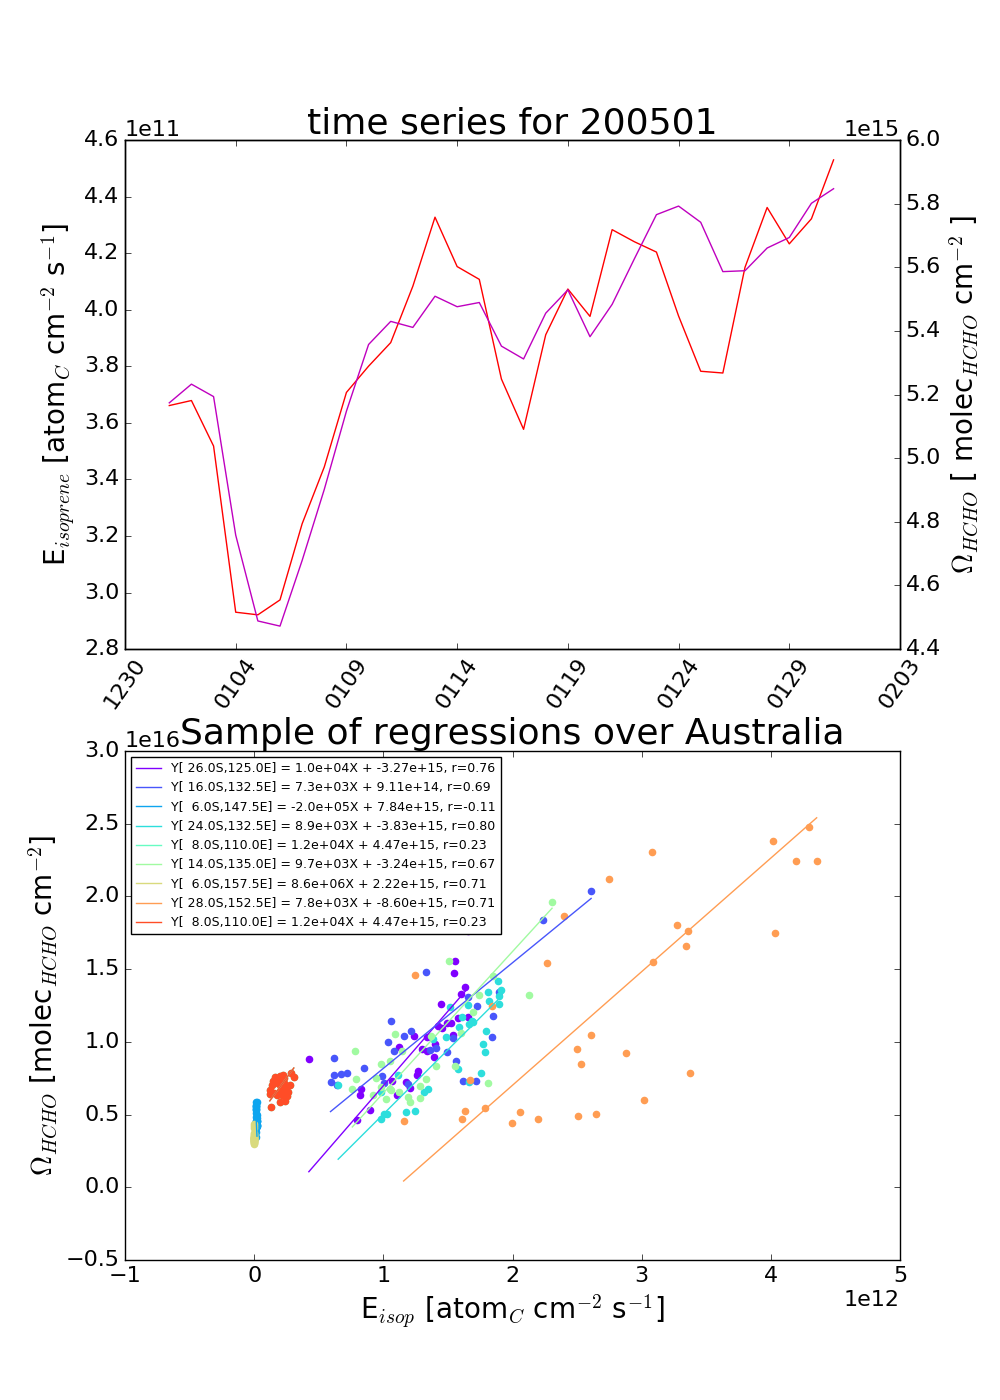
\includegraphics[width=\textwidth]{Figures/Isoprene/E_isop_vs_hcho_series_200501.png}
    %  \caption{%
    %    Top panel: isoprene emissions for January, 2005, shown in red, co-plotted with tropospheric hcho columns, shown in magenta.
    %    Both series are daily averages over Australia.
    %    Bottom panel: (RMA) linear regressions from between emissions of isoprene and tropospheric hcho columns, sampled randomly from the 2$^{\circ}$ by 2.5$^{\circ}$ latitude longitude gridboxes over Australia for the month of January (2005).
    %  }
    %  \label{BioIsop:method:calculation:fig_E_isop_vs_hcho_model_sample}
    %\end{figure}
    
    %% BACKGROUND calculation(s)
    There are two simple ways to determine the modelled background HCHO, one of which involves running the model with no isoprene emissions, which shows how much they alter vertical column HCHO.
    This is effective since we have assumed variation in HCHO columns only depends on isoprene emissions, so our background term is theoretically identical to the emission free simulated HCHO.
    The other way uses HCHO over the remote Pacific at matching latitudes and times, which emulates how the background is determined for the satellite measured HCHO.
    The difference between these two methods is negligible, so for consistency with satellite data, we determine backgrounds using the remote Pacific.
    Figure \ref{BioIsop:method:fig_background_hcho} shows GEOS-Chem total column HCHO with and without isoprene emissions along with amounts over the remote Pacific at the same latitudes.
    Background HCHO for any latitude in this thesis are calculated by averaging longitudinally (140\degr W to 160\degr W) the matching latitudes over the remote Pacific.
    %These backgrounds are used when creating the reference sector corrections for satellite measurements (in Section \ref{Model:omiRecalc:RSC}).
    %The background columns are longitudinally averaged from 140\degr W to 160\degr W.
    
    
    \mypic{Figures/OMI_link/GC/GC_background_hcho_200501.png}{Total column HCHO over Australia (left) and the remote Pacific region (right) using GEOS-Chem with (top) and without (bottom) isoprene emissions. }{\label{BioIsop:method:fig_background_hcho}}
    
    
  \subsection{Calculation of Emissions}
    \label{BioIsop:method:calculation}
   
    Top-down emissions estimates are calculated using OMHCHO (see Section \ref{Model:omhcho}) slant columns and an updated AMF calculated using code from Paul Palmer's group (see Section \ref{Model:omiRecalc:ppcode}).
    These emissions are referred to as the a postiori from here on, or $E_{OMI}$ in formulae.
    
    
    % First: outline of what we do
    As performed elsewhere \textcite[e.g.][]{Palmer2003, Millet2006, Bauwens2016}, we assume that HCHO and isoprene columns are in a steady state, with no horizontal transport.
    We also assume that isoprene is the only compound enhancing the HCHO levels, which requires that we filter out influence from fires, smoke, and anthropogenic emissions.
    Isoprene emissions are calculated using the linear relationship described in Section \ref{BioIsop:method:slope} using the modelled slope $S$ calculated in the prior section and satellite HCHO columns:
    \begin{eqnarray} \label{BioIsop:method:eqn_Enew}
      \Omega = & S \times E_{OMI} + \Omega_0 \notag \\
      E_{OMI} = & \frac{\Omega - \Omega{0}}{S}
    \end{eqnarray}
    This is the same equation \ref{BioIsop:method:slope:eqn_isop_to_hcho}, except now we use the modelled slope along with satellite HCHO ($\Omega$, and $\Omega_0$).
    $\Omega_0$ is calculated using measurements in the remote Pacific averaged monthly and longitudinally, for each $\Omega$, .
    This leaves $E_{OMI}$ as the only unknown once the satellite measurements are processed to match the temporal and horizontal resolution of $S$.
    Figure \ref{BioIsop:method:calculation:fig_E_isop_200501} shows the emissions calculated this way along with GEOS-Chem simulated emissions ($E_{GC}$) averaged over January, 2005.
    This figure gives a single month of output as an example, analysis of the full record is discussed in Section \ref{BioIsop:results}.
      
    \begin{figure}
      % Figure from Analyse_E_new.MEGAN_vs_E_new()
      \includegraphics[width=\textwidth]{Figures/OMI_link/Emiss/MEGAN_vs_E_VCC_PP_lr_20050101-20051231.png}
      \caption{%
        Top row is isoprene emissions for the month of January, in 2005, from GEOS-Chem and estimated from OMI respectively.
        Bottom row shows the absolute and relative differences between the two.
      }
      \label{BioIsop:method:calculation:fig_E_isop_200501}
    \end{figure}
    
    
    One potential issue is the low number of valid measurements, which occurs due to the higher zenith angles during winter or at higher latitudes.
    When calculating the $E_{OMI}$ from our modelled slope, negative emissions result wherever measured columns are lower than background amounts (as $E_{OMI} = \frac{\Omega - \Omega_0}{S}$).
    These are set to zero, which increases monthly Australian $E_{OMI}$ averages by TODO: $\sim X-Y$~\% with the highest increases occurring during (TODO winter?).
    
    Top-down emission rates calculated in this work are in units of molecules cm$^{-2}$ s$^{-1}$.
    In order to calculate the emissions in kg, each grid square is multiplied by the area, and then daily emissions are assumed to follow a sine wave peaking at $E_{OMI}$.
    Figure \ref{BioIsop:method:calculation:fig_daily_emissions_kg} shows how the daily approximation of total emitted isoprene per grid square is calculated.
    Daytime hours are estimated per month, from 14~hrs (Jan) to 10~hr(Jul).
    This approximation is required since OMI observations occur at midday, when isoprene emissions are at their diurnal peak.
    
    \mypicw{0.5\textwidth}{Figures/Emissions_per_day.png}{%
      Total daily isoprene emissions (in kg) is represented by the area under the sine wave.
    }{\label{BioIsop:method:calculation:fig_daily_emissions_kg}}
  
  
  \subsection{Accounting for smearing}
    \label{BioIsop:method:smearing}
    
    In high NO$_x$ ($ > \sim 1 $~ppb) environments where HCHO has a lifetime on the order of 30 minutes, it can be used to map isoprene emissions with spatial resolution from 10-100~kms \parencite{Palmer2003}.
    In low NO$_x$ conditions, isoprene has a longer lifetime (hours-days) and may form HCHO further from the source area.
    Horizontal transport \textit{smears} the HCHO signal so that source location would need to be calculated using wind speeds and loss rates \parencite{Palmer2001,Palmer2003}.
    Smearing is a measure of how much HCHO in a given grid box was produced from isoprene emitted in a different (upwind) grid box.
    Smearing affects emissions estimates as HCHO enhancements may be wrongly attributed as coming from areas downwind of where they occurred.
    Once smearing sensitive grid squares are filtered out, application of equation \ref{BioIsop:method:slope:eqn_isop_to_hcho} is used to estimate isoprene emissions across Australia.
    
    Over Australia NO$_x$ levels are generally not high enough to ensure quick HCHO formation and we must take care to account for resultant smearing.
    Smearing limits the horizontal resolution of the top-down inversion process used in this Thesis, as a finer resolution leads to increased issues with transport.
    The relatively coarse horizontal resolution (\lowhr) used by GEOS-Chem is advantageous in this aspect.
    Smearing has been analysed in various publications \parencite[e.g.][]{Martin2003, Palmer2003, Millet2006, Stavrakou2009, Marais2012, Barkley2013, Zhu2014, Wolfe2016, Surl2018}, and is often calculated using the method designed in \textcite{Palmer2003}.
    This involves using two almost identical model runs, one of which has isoprene emissions scaled globally by a factor (generally from 0.5 to 2).
    Another method \parencite[e.g.][]{Stavrakou2009} involves the analysis of an adjoint CTM, however this is computationally expensive and is not pursued here.
    
    %\textcite{Marais2012} additionally use airborn isoprene, MVK $+$ MACR (isoprene oxidation products), and HCHO measurements to check smearing in Africa where there is a sharp gradient of isoprene emitting vegetation from north to south.
    
    \subsubsection{Calculation of smearing}
      \label{BioIsop:method:smearing:calculation}
      
      % slope and yields
      In order to understand the smearing calculation the underlying equations and assumptions must first be understood.
      From Section \ref{BioIsop:method:slope}, equation \ref{BioIsop:method:slope:eqn_isop_to_hcho} we have the formulation of a modelled slope ($S$) being the yield of HCHO per C of emitted isoprene divided by HCHO loss rate per second ($S = \frac{Y_{isop}}{k_{HCHO}}$).
      % smearing defined from two runs of geos chem
      Using two runs of GEOS-Chem with isoprene emissions being the only difference we have:
      \begin{eqnarray}
        \label{BioIsop:method:smearing:calculation:eqn_runs}
        \begin{split}
        Run_1 :&  \Omega_{HCHO} = S E_{isop} + \Omega_0 \\
        Run_2 :&  \Omega_{HCHO}' = S' E_{isop}' + \Omega_0' 
        \end{split}
      \end{eqnarray}
      There are several assumptions which need to be understood, as these are what is tested by the smearing calculation.
      The initial assumption is that the system is in a steady state, with no transport of isoprene affecting HCHO columns, this is the basis for equations \ref{BioIsop:method:smearing:calculation:eqn_runs}.
      It is assumed that background values ($\Omega_0$) are from oxidation of methane and other long lived VOCs, so that $\Omega_0 = \Omega_0'$.
      Between these two runs we are only changing the $E$ term, we do not change any chemistry and so we can expect that the yield and loss rate is not changing between the two runs $S = S' = \frac{Y_{isop}}{k_{HCHO}}$
      %    \begin{eqnarray*}
      %      S = S' & = \frac{Y_{isop}}{k_{HCHO}} \\
      %      \Omega_0 & = \Omega_0'
      %    \end{eqnarray*}
      So that Equations \ref{BioIsop:method:smearing:calculation:eqn_runs} may be combined as follows:
      \begin{eqnarray}
        Run_1-Run_2 : \Omega_{HCHO} - \Omega_{HCHO}' = & S E_{isop} - S' E_{isop}' +\Omega_0 - \Omega_0' \notag \\
        \Omega_{HCHO} - \Omega_{HCHO}' = & S \left( E_{isop} - E_{isop}' \right) \notag \\
        \Delta \Omega_{HCHO} = & S \Delta E_{isop}  \notag \\
        & \hat{S} \equiv \frac{\Delta{\Omega_{HCHO}}}{\Delta E_{isop}} \approx \frac{Y_{isop}}{k_{HCHO}} \label{BioIsop:method:smearing:calculation:eqn_hats}
      \end{eqnarray}
      This allows the combination of outputs from the two runs to be used as a check against $\hat{S}$ being excessively different from expected values for $S$.
      %The modelled slope multiplied by the column HCHO loss rate ($k_{HCHO} = 1/\tau$) should approximate the HCHO yield from isoprene \parencite{Palmer2003, Barkley2013}.
      
      In order to filter potential smearing, a daily modelled value for $\hat{S} \approx Y_{isop}/k_{HCHO}$ is determined.
      By assuming midday HCHO lifetime typically falls within 1.5 to 4~hrs (as seen in the USA), and isoprene to HCHO yield (HCHO per isoprene carbon emitted) lies within the range 0.2 to 0.4 (scenarios estimated in \textcite{Palmer2003}): one can set a simple bound on $\hat{S}$ of $[0.2 \times 1.5, 0.4 \times 4]$~hrs or 1080 to 5760 seconds.
      As NO$_x$ levels across Australia are relatively low, the yield is likely lower than seen in \textcite{Palmer2003}: and here we reduce the bounds by 20\% and round to the nearest hundred to get a bounding range of 800 to 4600 for $\hat{S}$. 
      This range strikes a balance between unlikely modelled yields and how much data is lost to filtering.
      A better approximation of lifetimes for HCHO is required to properly account for seasonality and regional NO$_x$ concentrations.
      %Todo?: Show yield and lifetimes from caaba/mecca if possible
      Table \ref{BioIsop:method:smearing:tab_smearing_ranges} shows the smearing filters or typical slopes seen in other works.
      
      \begin{table}\begin{threeparttable}
          \caption{Smearing filters or slopes ($S$) seen in literature.}
          \begin{tabular}{ l | c  c  >{\centering\arraybackslash}p{5cm} } 
            \toprule
            Publication & min. (s) & max. (s) & Notes \\
            \midrule
            \textcite{Palmer2003}      & 1270 & 2090 & Slope ranges seen in north America summer \\
            \textcite{Marais2012}      &      & 4000 & Smearing limits for Africa \\
            \textcite{Barkley2013}$^a$ & 1300 & 1800 & Smearing limits for South America \\
            \textcite{Surl2018}        & 2200 & 4900 & Slope ranges seen in India \\
            In this Thesis             & 800  & 4600 & Smearing limits for Australia \\
            
            \bottomrule
          \end{tabular}
          \begin{tablenotes} 
            \item a: Assumed HCHO lifetime of 2.5 hours implies yields from 0.14 to 0.2 per C, consistent with box modelling.
            \item Slope ranges are observed or modelled $S$, while smearing limits are the applied acceptable limits for $S$ ranges. 
            %\item b: In this work the slopes are shown 
          \end{tablenotes}
          \label{BioIsop:method:smearing:tab_smearing_ranges}
        \end{threeparttable}\end{table}
      
      
      Similarly to smearing sensitivity calculations in \textcite{Marais2012}, we run GEOS-Chem with isoprene emissions halved, then calculate $\hat{S} = \frac{\Delta \Omega_{HCHO}}{\Delta E_{isop}} $ from Equation \ref{BioIsop:method:smearing:calculation:eqn_hats}.
      Here $\Delta$ represents the departure (daily over 1300-1400~LT) from default run values.
      If $\hat{S}$ sits outside an acceptable range then we remove that grid square day from both $S$ and subsequent $E_{isop}$ calculations.
      A relatively large change in $\Omega_{HCHO}$ compared to local emissions ($\hat{S}>4600$) suggests that HCHO is being formed from non-local isoprene emissions.
      Alternatively, a relatively low value of $\hat{S}$ ($\hat{S}<800$) suggests emissions from the local grid square are being exported before they form HCHO, meaning local HCHO levels are not due to local emissions.
      
      Smearing is sensitive to how E$_{isop}$ is determined, Figure \ref{BioIsop:method:smearing:fig_smearing_def_2005} shows smearing over two seasons.
      Isoprene emissions (E$_{isop}$) is defined in two ways in this figure: left column from daily averaged flux, and right column from and midday (1300-1400~LT) flux. 
      Essentially the midday isoprene emissions are at the peak of their daily cycle (shown later in Figure \ref{BioIsop:method:scaled:megan_diurnal}) which means the effect of smearing is relatively smaller during these hours.
      
      
      \mypic{/Figures/OMI_link/Filters/smearing_definitions_2005.png}{%
        Smearing ($\hat{S}$, see text) in summer (DJF, top row) and winter (JJA, bottom row) using averaged isoprene emissions daily (left column) and 1300-1400~LT (right column). 
        The scale changes between left and right columns.}{\label{BioIsop:method:smearing:fig_smearing_def_2005}}
      
      
      % Marais 2012 also look at average windspeed and best hcho-isop corelation when hcho is shifted by 0.5 degrees, don't think I can do that with 2.5 degree resolution
      % Marais compare smearing with model estimated yield "

    \subsubsection{Sensitivity to smearing}
    
      
      %TODO: Plots of S hat showing worst smearing affected areas per season.
      Figure TODO: shows averaged isoprene emissions with added markers showing when the threshold of 800-4600 affects at least one day within the season (cyan or pink diamonds) and where it removes all data for that gridbox (blue or red x).
      Smearing can be dependent on local or regional weather patterns, as greater wind speeds will reduce the time any emitted compound stays within the local grid box.
      As such smearing can vary greatly both spatially and temporally.
      Large smearing values can be seen near coastlines as only a fraction of these grid squares actually emit isoprene, which makes transported isoprene relatively more important in these gridboxes.
      During summer data-loss from smearing is only minor (todo: Y\%), however data-loss peaks in winter (TODO X \%), especially in higher southern latitudes.
      
      
      % TODO: figure out this paragraphs numbers, make plot
      When limiting smearing ($\hat{S}$) to within 800-4600~s, GEOS-Chem correlation between isoprene emissions and HCHO columns should improve (TODO analysis). 
      A problem arises due to the loss of data used to create monthly grid square regressions.
      $S$ and associated regression coefficients ($r$) are calculated monthly, if $r<0.4$ then the regression is calculated using multiple years of data for that month.
      This multiple year regression is discarded completely if it also fails the $r<0.4$ threshold, leaving no slope for the grid square for the month.
      %potentially where the 95\% confidence interval min and max ratio is too high (too wide).
      Figure TODO shows GEOS-Chem midday HCHO columns compared against GEOS-Chem emissions of isoprene, over land squares with (red) and without (grey) filtering for smearing.
      This smearing range captures isoprene to HCHO yields of around 0.16 to 0.32 C per C if HCHO lifetime is assumed to lie within 1.5 to 4 hours.
      These ranges mean we only use data which is not outside the feasible bounds of yields or lifetimes in Australia.
    
    \subsubsection{Smearing length scale}
    
      %TODO: Actually calculate smearing length
      The expected horizontal transport (prior to reaction) of a precursor can be calculated using the smearing length \parencite{Palmer2003}.
      The distance travelled ($L$) downwind ($d$) by a precursor ($i$) before forming HCHO can be estimated through:
      \begin{equation*}
        L_{d,i} = \frac{U}{k_i - k_{HCHO}} \ln{ \left( \frac{k_i}{k_{HCHO}} \right) }
      \end{equation*}
      where $U$ is wind-speed.
      \textcite{Palmer2003} further define a smearing length scale: $L_{s,i}$ as the distance downwind where a fraction (1 - $1/e$) of the precursor is completely transformed into HCHO.
      This equation uses the initial VOC column concentration ($[VOC]_0$) at the point of emission and mass balance equations as follows:
      %TODO: Add intermediate steps
      \begin{equation}
      \frac{1}{k_{HCHO}-k_i} \left( k_{HCHO} \exp{ \left[ \frac{-k_i L_{s,i}}{U} \right]} -k_i \exp{ \left[ \frac{-k_{HCHO} L_{s,i}}{U} \right]} \right) = \frac{1}{e} 
      \end{equation}
      with limiting values $L_{s,i} \rightarrow U/k_i$ for $k_i << k_{HCHO}$, and $L_{s,i} \rightarrow U/k_{HCHO}$ for $k_{HCHO} << k_i$.
      Figure TODO: shows a rough estimate of isoprene smearing length($L_{isop}$) in Australia using wind speeds from TODO:, and reaction rates $k_{isop}$, $k_{HCHO}$ from GEOS-Chem.
      %TODO make this plot!
      
      % Discussion of HCHO and isoprene lifetimes/yields 
      The half-life of HCHO %to photo-oxidation with hydroxyl radicals 
      is around 1~hr depending on environmental conditions \parencite{WHO_hcho_guidelines_2010}.
      This would make the expected lifetime ($\tau = \text{half-life}/\ln{2}$) around 1.4 hours.
      Over the majority of Australia conditions are relatively clean (low NO$_x$) which extends the expected lifetime.
      The estimated loss rate of HCHO in GEOS-Chem %approximately ranges from 1e6 to 3e6 mol cm$^{-3}$ s${-1}$, 
      is up to three times higher in summer and along the north and eastern regions associated with denser forest regions, when compared against other regions.
      This is largely due to loss rates being proportional to concentrations.
      % WHAT importance does hcho lifetime have in regards to smearing and scale length?
      
      % WHEN CALCULATING SMEARING SCALE MAYBE ASSUME ONE OF THESE 
      Isoprene yields can vary greatly, and are dependent on NO$_x$ levels, some prior literaature values are shown in Table \ref{BioIsop:method:tab_VOCLiteratureYields}.
      Increasing NO$_x$ from 0.1~ppbv to 2.0~ppbv can triple the prompt yield of HCHO, %from 0.3 to 0.9 ppbv ppbv$^{-1}$
      due to isoprene, and double background HCHO \parencite{Wolfe2016}.
      
      %Conversions between HCHO per unit C yield and molar \% yield from species X are given by the equation $ Y_{molar \%} = 100 \times C_X \times Y_{HCHO \,C^{-1}}$, where $C_X$ is how many carbon are within species X (5 for isoprene).
      %For instance a 200\% molar yield of HCHO from isoprene implies 1 mole of C$_5$H$_8$ becomes 2 mole HCHO which is a 0.4 HCHO per unit C yield.
      %      
      % yields from Atkinsen2003
      %isoprene
      %0.63 0.10 Tuazon and Atkinson (1990a)
      %0.57 0.06 Miyoshi et al. (1994)
      % a-pinene
      %0.23 0.09 Noziere et al. (1999a)
      %0.19 0.05 Orlando et al. (2000)
      % b-pinene
      %0.54 0.05 Hatakeyama et al. (1991)
      %0.45 0.08 Orlando et al. (2000)
      
      % molar HCHO yield per unit carbon equal to HCHO molar percent yield(per carbon)? or some conversion?
      \begin{table} \begin{threeparttable}
          \caption{ Isoprene to HCHO yields and lifetime.}% against oxidation by OH. }
          \begin{tabular}{  l  l  l  l  }
            \toprule
            HCHO Yield    & Lifetime     & NO$_x$ background & Source   \\
            (molar \% )   &              &                   &          \\
            \midrule 
            315$\pm$50      &            & High          & a        \\ 
            285$\pm$30      &            & High          & a        \\ 
            225             & 35 min     & High          & b        \\ % Done
            150             &            & Low           & b        \\ % Done
            150             &            & Low           & d        \\
            450             &            & High          & d        \\
            235             &            & 1~ppbv        & e        \\
            150             &            & 0.1~ppbv      & e        \\
            %          $\alpha$-Pinene & 28$\pm$3        &        & Low                & c        \\ 
            %          & X$\pm$3         &        & X                  & d        \\ 
            %          & 230$\pm$90      &        & High        & a        \\ 
            %          & 190$\pm$50      &        & High        & a        \\ 
            %          & 19              & 1 hour &              & b        \\ % Done
            %          & 210             &        & 1~ppbv        & e        \\
            %          & 70              &        & 0.1~ppbv      & e        \\
            %          $\beta$-Pinene  & 65$\pm$6        &        & Low           & c      \\ 
            %          & X$\pm$3         &        & X             & d      \\ 
            %          & 540$\pm$50      &        & High          & a     \\ 
            %          & 450$\pm$80      &        & High          & a      \\ 
            %          & 45              & 40 min &              & b      \\ % Done
            %          Methane 	      & 100             & 1 year  &             & b     \\ 
            %          Ethane          & 180             & 10 days &             & b     \\ 
            %          Propane         & 60              & 2 days  &             & b     \\ 
            %          Methylbutanol   & .13(per C)    & 1 hour  &             & b     \\ 
            %          HCHO            & 100             & 2 hour  &             & b     \\ 
            %          Acetone         & .67(per C)      & 10 days &             & b     \\ 
            %          Methanol        & 100             & 2 days  &             & b     \\ %Done
            \bottomrule
          \end{tabular}
          \begin{tablenotes} % \item makes new lines
            \item a \textcite{AtkinsonArey2003}: Table 2, Yield from Isoprene reaction with OH, two values are from two referenced papers therein.
            \item b \textcite{Palmer2003}: lifetimes assume [OH] is 1e15 mol cm$^{-3}$.
            \item c \parencite{Lee2006}: Calculated through change in concentration of parent and product linear least squares regression.
            Estimates assume 20$^\circ$~C conditions.
            \item d \textcite{Wolfe2016}: ``prompt yield'': change in HCHO per change in ISOP$_0$.
            $[ISOP]_0=[ISOP]\exp(k_1[\mathrm{OH}]t)$; where $k_1$ is first order loss rate.
            Effectively relates HCHO abundance with isoprene emission strength.
            \item e \textcite{Dufour2009}: One-day yields from oxidation modelled by CHIMERE, using MCM reference scheme.
            %\item f Calculated using PTR-MS and iWAS on SENEX campaign data.
          \end{tablenotes}
          \label{BioIsop:method:tab_VOCLiteratureYields}
        \end{threeparttable} \end{table}
      
      GEOS-Chem daily averaged HCHO lifetime ($\tau$) is shown for 2005 in Figure \ref{BioIsop:method:smearing:fig_tau_GC_2005}.
      This lifetime $\tau$ is calculated using daily averaged surface loss rates ($L_{HCHO}$) and concentrations of HCHO:
      \begin{equation*}
      \tau = \frac{[HCHO]}{L_{HCHO}}
      \end{equation*}
      The expected lifetime of HCHO is determined by assuming loss is linear (first order) and dividing grid box daily averaged concentrations of GEOS-Chem HCHO ($[HCHO]$ in molecules cm$^{-3}$) by their modelled losses ($L_{HCHO}$ in molecules cm$^{-3}$ s$^{-1}$).
      For each grid square over Australia this daily averaged surface lifetime in summer (Jan., Feb.) and winter (Jul., Aug.) is shown in Figure \ref{BioIsop:method:smearing:fig_tau_GC_2005}.
      Additionally lifetimes coloured by land grid squares (dots in top right panel) are shown over time in the bottom panel.
      Note that this figure shows the daily averaged lifetime, but further analysis and calculations are based on mid-day (13:00-14:00~LT) values when the lifetime will be significantly shorter. 
      This figure highlights the seasonal nature of HCHO lifetime, although midday numbers are expected to have less seasonality than shown here, since shorter days will not affect midday lifetimes.
      Another highlighted issue is the potential latitudinal dependence of HCHO lifetimes, since there is less total insolation leading to lower HCHO loss rates at higher latitudes.
      The overall takeaway is that the accuracy and utility of any top down HCHO precursor estimation technique will be limited by both season and potentially latitude.
      These limitations are due to both data availability (as satellite HCHO suffers from high zenith angles) and spatial smearing (from HCHO lifetimes which increase with lower insolation and temperature).
      
      \mypic{/Figures/OMI_link/Filters/tau_2005.png}{%
        Top left, right: summer (Jan., Feb.) and winter (JJA) averaged daily surface HCHO lifetime ($\tau$). Bottom panel: $\tau$ over the year, coloured by grid square (see dots in top right panel).
      }{\label{BioIsop:method:smearing:fig_tau_GC_2005}}
      
    
    \subsubsection{NOx dependence}
      
      Isoprene production of HCHO depends on several factors, importantly NO$_x$ levels directly affect the fate of VOCs in the atmosphere.
      Isoprene first reacts with the hydroxy radical, producing an organic peroxy radical (RO$_2$).
      At higher NO mixing ratios (at least a few hundred pptv), RO$_2$ react mostly with NO. 
      At low NO (less than 50~pptv), RO$_2$ is more likely to either isomerise, or react with HO$_2$, or another RO$_2$.
      In low NO$_x$ environments, reported HCHO yields from isoprene are around 0.2 - 0.3 C per C, while in high NO$_x$ environments this value becomes two to three times higher \parencite{Palmer2003, Wolfe2016}.
      %\textcite{Wolfe2016} also see background HCHO doubling in high NO$_x$ regions.
      %\textcite{Wolfe2016} determine that going from NO$_X = 0.1$ to $2.0$ ppbv triples the prompt yield of HCHO, from 0.3 to 0.9 ppbv ppbv$^{-1}$ due to isoprene, while the background HCHO doubles.

      
      NO$_2$ from the OMNO2d product provides daily mid-day measurements which we compare to output from GEOS-Chem NO$_2$ (see Section \ref{Model:GC:NOx}).
      %\textcite{Travis2016} show how NO$_x$ can be used to examine model bias in ozone (potentially due to NO$_2$ bias) over the USA.
      The effect of NO$_2$ on smearing can be seen in Figure \ref{BiogIsop:Method:smearing:fig_smearing_vs_nox}.
      This plot shows how smearing over Australia compares to satellite NO$_2$, with smearing distributions binned by NO$_2$ both with and without applying a filter for smearing.
      At lower NO$_2$ levels the smearing is often 2-4 orders of magnitude above the upper threshold. 
      This abruptly decreases at around $5 \times 10^{14} $~molec cm$^{-2}$ NO$_2$.
      There is also a higher number of data points below the lower threshold before that same NO$_2$ level, suggesting that transport is a bigger issue at NO$_2 < 5 \times 10^{14} $~molec cm$^{-2}$. 
      
      %% FIGURE SHOWS SMEARING BINNED BY NOX
      % Figure made in test_filters.smearing_nox() 
      \mypic{Figures/OMI_link/Filters/smearing_nox_200501.png}{%
        Top left: OMNO2d tropospheric NO$_2$ columns (NO$_2$: molec cm$^{-2}$) averaged into \lowhr horizontal bins for Jan, 2005.
        Right: Scatter plot of NO$_2$ against smearing calculations from GEOS-Chem ($\hat{S}$), with points above and below the smearing threshold range of 900-5200~s coloured red and blue respectively. 
        Points are binned by NO$_2$ with and without the smearing filter applied (orange and magenta respectively).
        Overplotted is the mean and standard deviation (error bars) within each bin. 
        Due to the logarithmic Y scale we only show the positive direction of standard deviations for unfiltered data.
        Bottom left: Daily NO$_2$ scattered against smearing with (magenta) and without (orange) applying the smearing filter. This plot is a zoomed out version of the right panel.
      }{\label{BiogIsop:Method:smearing:fig_smearing_vs_nox}}
      

  \subsection{Running GEOS-Chem using a postiori emissions}
  \label{BioIsop:method:scaled}
    
    After creating $E_{isop}$, our a postiori isoprene emissions estimate, we run GEOS-Chem again with biogenic emissions scaled to match the new estimate. 
    First all the new midday (13:00-14:00~LT) emissions (per grid box) and forming a multi-year monthly mean, which can be compared to the unaltered GEOS-Chem equivalent.
    A monthly factor ($\alpha$ at \lowhr) that scales MEGAN towards our top-down estimate is then read by the emissions module in GEOS-Chem, and applied whenever isoprene emissions are calculated.
    %Initially a run of GEOS-Chem using no chemistry it performed is order to quickly retrieve hourly averaged isoprene emissions.
    This scaling allows the shorter time-scale variability and dependencies to be retained, while moving the monthly mean value towards the multi-year monthly averaged a postiori.
    Short time-scale variability is largely due to meteorological parameters such as temperature and light, etc..
    TODO: Figure X shows an example of this process for January: with the multi-year average emissions mapped over Australia (rows one and two) being used to create the $\alpha$ in the third row.
    
    
    The scaling factor $\alpha$ is the ratio between the multi-year averaged monthly emissions from GEOS-Chem $E_{GC}$ and the a postiori $E_{OMI}$: 
    \begin{equation} \label{BioIsop:method:scaled:eqn_alpha}
        \alpha = \frac{E_{OMI}}{E_{GC}}
    \end{equation}
    A small modification of GEOS-chem source code multiplies biogenic emissions by $\alpha$ for each grid-square based on the default emission factors and meteorology.
    Initially $\alpha$ is uniformly set to 1 globally.
    Where we have top down emissions and $E_{GC}$ is non-zero, we can set $\alpha$ using Equation \ref{BioIsop:method:scaled:eqn_alpha}.
    Missing values for $\alpha$ when $E_{GC}$ are zero are an issue, however this is negligible since the dominant discrepancies between estimates occurs during summer when high emission rates are overestimated.
    Figure \ref{BioIsop:method:scaled:fig_alpha_mya_series} shows $\alpha$ for the average January and June over 2005-2012, along with a time series of $E_{GC}$ and $E_{OMI}$ and $\alpha$ calculated for Sydney, and their multi-year seasonal average.
    
    % Figure from TODO:???
    % UPDATE TO a priori and a postiori
    \mypic{Figures/OMI_link/new_emiss/alpha_mya.png}{%
      Row 1: $\alpha$ for the average January (left) and June (right) over 2005-2012.
      Row 2: $E_{GC}$ (xxx, left axis), $E_{OMI}$ (xxx, left axis), and  $\alpha$(black, right axis) multi-year monthly averages calculated for Sydney.
      Row 3: Monthly averages of the same terms in Row 2.}{\label{BioIsop:method:scaled:fig_alpha_mya_series}}

\section{Results}
  \label{BioIsop:results}
  
  Australia is roughly $7.7 \times 10^6$ km$^{2}$, with heterogeneous environmental conditions.
  The results presented in this section are frequently split into five regions which are differentiated by colour, as shown in Figure \ref{BioIsop:results:fig_subregions}.
  
  % figure from Analysis_E_isop.py.show_subregions()
  \mypic{Figures/OMI_link/subregions.png}{%
    Sub-regions used in subsequent figures.
    Australia-wide averages will be black or grey, while averages from within the coloured rectangles will match the colour shown here.
  }{\label{BioIsop:results:fig_subregions}}
  
  
  \subsection{Updated emissions}
    \label{BioIsop:results:emissions}
    
    Figure \ref{BioIsop:results:emissions:fig_time_series_vs_megan} shows a priori emissions over Australia (todo column 1) and the updated emissions calculated using OMI (column 2: a postiori).
    The first row shows the time series (daily midday averages) and the final row shows the absolute differences (a priori - a postiori).
    This figure is repeated using monthly means (of the daily midday estimates) in Figure \ref{BioIsop:results:emissions:fig_time_series_vs_megan_monthly}.
    Over the entirety of Australia the seasonal cycle of emissions is shown to be overestimated by the a priori.
    The difference between a priori and a postiori estimates differs between regions, and some noise can be seen in the monthly time series due to data loss (TODO: check data counts).
    While most regions generally adhere to this behaviour of overestimation, the northern region of Australia follows a different cycle of bias.
    Northern Australia appears to be overestimated throughout the year, however occasional low points occur in summer in which the a priori is near to or lower than the a postiori.
    One potential reason is the onset of the wet season (November-April) which disrupts the ecosystems and limits satellite measurement through increased cloud coverage.
    
    % TODO: Update to have apriori on left, a postiori on right
    % Figure from Analyse_E_isop.py -> E_regional_time_series()
    \mypic{Figures/OMI_link/Emiss/E_zones_PP_lr.png}{%
      Biogenic emissions of isoprene from GEOS-Chem (running MEGAN), which is our a priori in column 1, and the emissions calculated using the OMI top down inversion, which is our a postiori in column 2.
      %Row 1: overall averaged daily midday emission rates, from 1, Jan, 2005 to 1, May, 2013.
      Row 1: time series of daily midday averages for all of Australia along with several subregions (shown in row 1). 
      The black lines and grey areas show the Australian mean and inter-quartile range respectively, while the coloured lines show the mean within subregions as shown in Figure \ref{BioIsop:results:fig_subregions}.
      The overall regional averages are shown at the end of the time series by horizontal lines.
      Row 2: Absolute differences: a priori - a postiori.
      TODO: remove spines along top and middle of top row
    }{\label{BioIsop:results:emissions:fig_time_series_vs_megan}}
    
    % also Analyse_E_isop.E_regional_time_series()
    \mypic{Figures/OMI_link/Emiss/E_zones_PP_monthly_lr.png}{ %
      As Figure \ref{BioIsop:results:emissions:fig_time_series_vs_megan} using monthly medians of the daily midday emissions estimates.
    }{\label{BioIsop:results:emissions:fig_time_series_vs_megan_monthly}}
    
    Figure \ref{BioIsop:results:emissions:fig_megan_vs_Enew_regional_mya} shows the multi-year monthly mean and IQR of daily midday isoprene emissions estimates, averaged regionally (see Figure \ref{BioIsop:results:fig_subregions}). 
    Generally months outside of May to August show the a postiori lower than the a priori, except in the south eastern region.
    Here the difference is only prominent during February, TODO check if this may be because of data point counts.
    %JENNY NOTE:
    TODO: Which regions show best correlation? Worst? Why might that be, and what does it mean?
    
    % Figure from Analyse_E_isop.py -> E_regional_multiyear()
    % TODO update titles and add Y axis, update legend
    % TODO run over 2005-2012
    \mypic{Figures/OMI_link/Emiss/E_zones_multiyear_PP_lr.png}{ %
      The multi-year monthly mean (lines) and IQR (shaded) of midday (13:00-14-00~LT) isoprene emissions estimates. 
      %Estimates come from MEGAN run by GEOS-Chem (E$_{GC}$), and the OMI top-down technique (E$_{OMI}$).
      A priori emissions are shown by the dashed lines and hatched shaded areas show the IQR.
      A postiori emissions are shown using the solid lines, with IQR shown by unhatched shaded areas.
      Colours denote the region over which the monthly average was taken, as in Figure \ref{BioIsop:results:fig_subregions}.
    }{\label{BioIsop:results:emissions:fig_megan_vs_Enew_regional_mya}}
    
    Figures \ref{BioIsop:results:emissions:fig_daily_egressions} and \ref{BioIsop:results:emissions:fig_monthly_egressions} show how the distributions of a postiori emissions compare to the a priori in each region during summer months (DJF) with zeros removed from both distributions. % zeros or negatives in top-down estimate are from hcho lower than background
    Figure \ref{BioIsop:results:emissions:fig_daily_egressions} shows the daily midday distributions, binned hexagonally to show data-point frequency.
    There is only weak correlation between daily estimations, and the distributions are quite different with more variance shown by the a priori.
    This is likely due to filtering applied to a postiori emissions, and missing satellite data (e.g. whenever cloud coverage exceeds 40\%).
    Figure \ref{BioIsop:results:emissions:fig_monthly_egressions} displays the regressions between monthly averages of the same data. 
    In the monthly averages a stronger correlation is apparent, with regression coefficients ranging from 0.48 to 0.78 across regions.
    The portion of this correlation due to seasonality is examined by re-running the regression after subtracting the multi-year monthly average from each dataset.
    TODO: run regression after removing seasonal average and see how r and slope are affected.
    
    \mypic{Figures/OMI_link/Emiss/daily_Egressions.png}{%
      Scatter plot (binned hexagonally to show data-point frequency) along with the distributions of MEGAN (y axis) and the top down estimate (x axis).
      This figure is based on summer (DJF) midday values over multiple years.
      Coloured by regions shown in Figure \ref{BioIsop:results:fig_subregions}.
    }{\label{BioIsop:results:emissions:fig_daily_egressions}}
    
    % UPDATE: fix Y axis labels -> a priori, X axis -> a postiori, add units, remove negative axes, REMOVE legend point marker
    % Figure from Analyse_E_isop.distributions_comparison_regional()
    \mypic{Figures/OMI_link/Emiss/monthly_Egressions.png}{%
      Scatter plot of a priori emissions against a postiori using monthly averaged grid squares as regression datapoints.
      Data points are created using monthly averages (of midday emissions) for each grid box for each month of summer (DJF) within each region shown.
      Multiple years of data are used, meaning if a region has 10 grid boxes, the 8 years of data will add up to $10 \times 3 \times 8 = 240$ data points minus filtered and zero emission squares.
      Plots are coloured by regions matching those shown in Figure \ref{BioIsop:results:fig_subregions}.
      The linear best fit regression is inset into each plot along with the line equation and regression coefficient.
    }{\label{BioIsop:results:emissions:fig_monthly_egressions}}
    
    After running GEOS-Chem with isoprene emission scaled to match the a postiori, the first preliminary check on the modelled output checks total column HCHO ($\Omega_{HCHO}$) over January in 2005 in Figure \ref{BioIsop:results:emissions:fig_prelim_new_emiss_HCHO}.
    In every region the new modelled $\Omega_{HCHO}$ is closer to the satellite measured amounts with biases lowering from 50-120\% down to 30-50\%.
    
    % figure from initial version of tests/test_new_emissions.hcho_ozone_series
    \mypic{Figures/OMI_link/new_emiss/HCHO_total_columns_20050101_20050131.png}{%
      Daily mean total column HCHO amounts from GEOS-Chem with (new emissions run) and without (tropchem run) a postiori scaled isoprene emissions, along with the original OMI HCHO columns.
      Each row shows the average over regions in Figure \ref{BioIsop:results:fig_subregions}. }{\label{BioIsop:results:emissions:fig_prelim_new_emiss_HCHO}}
    
    
  \subsection{A postiori GEOS-Chem results}
  \label{BioIsop:results:new_emiss}
    
    This section describes how outputs from GEOS-Chem change after applying a scaling factor $\alpha$ (see Section \ref{BioIsop:method:scaled}) to biogenic isoprene emissions.
    Here we need to be careful of notation, unscaled GEOS-Chem biogenic emissions are the a priori, top down midday emissions are the a postiori, and emissions from the scaled GEOS-Chem run are denoted E$^{\alpha}_{GC}$.
    
    Figure \ref{BioIsop:method:scaled:megan_diurnal} shows the multi-year monthly mean daily cycle of isoprene emissions from GEOS-Chem, along with the top-down midday estimate, for an example grid box located 2.5~\degr~ W of Sydney.
    TODO: Analysis of this and lead into more analysis of differences
    
    \mypic{Figures/OMI_link/Emiss/MEGAN_monthly_daycycle.png}{ %
      The diurnal cycle of MEGAN emissions averaged by month over 1, Jan, 2005 to TODO, 2013 are shown with lines, while top-down emissions estimates are shown with plus symbols.
      MEGAN emissions are estimated hourly per \lowhr horizontal grid box, shown here are the area averages (denoted by colour, see Figure \ref{BioIsop:results:fig_subregions}).
      Top-down estimates are similarly grouped by colour, and shown at the 13:00~LT mark for each month.
      }{\label{BioIsop:method:scaled:megan_diurnal}}
      
    TODO: how isoprene is linked to ozone in modelling 
    Figure \ref{Conclusions:ozone:fig_new_emiss_series_O3} shows surface level (up to $\sim 150$~m altitude) ozone concentration over 2005 before and after scaling modelled isoprene emissions.
    Reducing isoprene emissions lowers surface ozone concentrations by TODO: XX to YY \% in summer, and XX to YY \% in winter.
    The direct correlation between reduced emissions and surface ozone (Figure TODO) is more or less clear monthly, and using multiple years enhances/reduces the relationship.
    A look at the regression using only summer data reveals a stronger/weaker relationship, analyse per region (TODO).
  
  \subsection{Trends}
    \label{BioIsop:results:trends}
    
    TODO: Summary of how the VOC NOX Ozone dynamic is changing over time, including how they are linked
    
    
    Plot time series of isoprene emissions for each region pre and post change
    subtract seasonal mya cycle and show trend and p value for trend being non-zero.
    Figure \ref{BioIsop:results:trends:fig_emission_anomalies} shows a priori and a postiori midday emissions for each region, with the respective multiyear monthly mean subtracted to detect any trend over 2005 - 2012.
    First each region is spatially averaged to form a daily time series of midday emission rates, this is re-sampled to a monthly average and then the multiyear monthly mean is subtracted from this before a linear regression is performed to look for any significant trend.
    Additionally any anomaly which is greater than 3 standard deviations from the mean is removed (these points can be seen as crosses in Figure \ref{BioIsop:results:trends:fig_emission_anomalies}).
    A trend is considered significant if the 95\% confidence interval of the gradient does not include 0.
    We see the a priori trend is negative for all regions, which is the reverse of the a postiori in all but the south eastern region.
    The trends in a postiori emissions suggest growth of $\sim 8-16\%$ of the annual average emission rate per year over the period, except in south eastern Australia where a $\sim 13\%$ decline is seen.
    
    \mypic{Figures/OMI_link/Emiss/trend_E.png}{%
      A priori (row 1) and a postiori (row 2) emissions anomaly from multiyear monthly mean, split by region (see Figure \ref{BioIsop:results:fig_subregions}).
      }{\label{BioIsop:results:trends:fig_emission_anomalies}}
      
    
    TODO: how HCHO is changing over the period
    Plot: time series pre and post isoprene changes as well as OMI for each region.
    subtract seasonal mya cycle and show trend and p value for trend being non-zero.
    
    TODO: how surface ozone is changing over the period
    plot: time series of ozone pre and post isop change
    subtract seasonal mya cycle and show trend and p value for trend being non-zero.
    
    \begin{table}\begin{threeparttable}
      \caption{Regional 95\% confidence interval of slope from linear regression of anomalies}
      \begin{tabular}{ l  c  c  c} 
        \toprule
        region & midday isoprene emissions & ozone & hcho \\
        \midrule
        \textbf{a priori emissions}$^a$ & & & \\
        Aus & [ X, Y] & [X, Y] & [X, Y] \\ 
        \midrule
        \textbf{a postiori emissions}$^b$ & & & \\
        Aus & [ X, Y] & [X, Y] & [X, Y] \\ 
        \bottomrule
      \end{tabular}
      \begin{tablenotes} 
        \item a: GEOS-Chem output using default isoprene emissions
        \item b: GEOS-Chem output (except for midday isoprene emissions) using scaled isoprene emissions
      \end{tablenotes}
    \end{threeparttable}\end{table}
    
  \subsection{Literature comparisons}
    
    % 
    When comparing the GEOS-Chem (which runs MEGAN) emissions to those calculated using our top-down inversion, we see a decrease of around 29\tgpyr ($66\%)$.
    \textcite{Sindelarova2014} see a 41\tgpyr decrease in Australia when introducing soil moisture parameterisation.
    Table \ref{BioIsop:results:emissions:tab_emissions_Tg} shows yearly isoprene emissions from this work and some other works for Australia.
    Figure \ref{BioIsop:results:emissions:fig_tga_comparison_map} shows how this decrease is distributed spatially, with $E_{GC}$ and $E_{OMI}$ in \tgpyr calculated as a multi-year mean.
    Across all of Australia we see large reductions of total emissions using the new top-down estimate.
    
    \mypic{Figures/OMI_link/Emiss/tga_map.png}{%
      Top row: multi-year mean emissions in \tgpyr from $E_{GC}$ (GEOS-Chem; running MEGAN) and $E_{OMI}$ (top-down emissions) respectively.
      $E_{OMI}$ uses an assumed sinusoidal daily cycle, with daylight hours perscribed for each month: see Section \ref{BioIsop:method:calculation}).
      Bottom left and right shows the absolute and relative differences respectively.}{\label{BioIsop:results:emissions:fig_tga_comparison_map}}
    
    
    %TODO: Update with 2005-2013 rather than just 2005-2007
    %global MEGAN: 471.518577725
    %aus MEGAN: 45.4326831613
    %aus OMI  : 16.4731027389
    
    \begin{table}\begin{threeparttable}
      \caption{Isoprene emissions (Tg/yr)}
      \begin{tabular}{ l  c  >{\arraybackslash}p{10cm} } 
        \toprule
        Australia & notes \\
        \midrule
        43(2) & a) GEOS-Chem: 2005-2010 \\ % 445(18) globally
        19(2) & b) Top-down: 2005-2010 \\
        26-94 & c) \textcite{Bauwens2016}: 2005-2013\\
        %&  535 & \textcite{Guenther2012}: \\
        %&  594 & \textcite{Sindelarova2014}: \\
        %26-94 & 272-570 & c) \textcite{Bauwens2016}: 2005-2013\\
        \bottomrule
      \end{tabular}
      \begin{tablenotes} 
        \item a: MEGAN diagnostics based on 3-hourly averages
        \item b: Based on daily peak emissions integrated over a sinusoidal daily curve
        \item c: Range shown here based on 3 different models and one top-down inversion
      \end{tablenotes}
      \label{BioIsop:results:emissions:tab_emissions_Tg}
    \end{threeparttable}\end{table}
  
  \subsection{Comparison with available measurements}
    \label{BioIsop:results:measurements}
    TODO: % TODO: campaign analysis compared to GEOS-Chem
    Analyse comparison of gridbox with campaigns of measurements
    
    Comparison between ground-based measurements and large (\lowhr) averaged grid squares suffers from representation error.
    Figure \ref{BioIsop:results:measurements:fig_gridbox} shows the SPS and MUMBA measurement sites, along with an outline of the \lowhr model grid box.
    The grid box is the area over which GEOS-Chem outputs are averaged, a rectangle with edge lengths of roughly 200~km$^{2}$.
    The urban footprint of Sydney and Wollongong are clearly shown, along with some ocean, forest, and rural regions, which will all affect the model output and other calculations averaged here.
    Due to high uncertainty in components of the top-down emissions estimate, temporal resolution is also limited.
    MUMBA, SPS1 and SPS2 each provide relatively few data points, which are compared against surface level concentrations from GEOS-Chem before and after scaling the biogenic emissions.
    %campaigns measured isoprene concentrations while our estimate is of emissions.
    
    %figure from Jenny
    \mypic{Figures/gridmapsmall_sites.png}{% 
      Gridbox at \lowhr containing SPS, and MUMBA campaign data.}{\label{BioIsop:results:measurements:fig_gridbox}}
    
    Figure \ref{Model:datasets:SPS:fig_GC_comparison} shows GEOS-Chem output in the grid square containing Sydney overlaid on SPS measurement data.
    Superficially the comparison is not too bad between these two datasets.
    %, however GEOS-Chem output is the daily average over \lowhr (latitude by longitude).
    This figure shows at a glance how the measurements compare to modelled data, and also the limited nature of the temporal and spatial scale of available measurements.
    TODO: if possible use midday isoprene multi-year averages, and error bars? then update discussion.
    The SPS data is point-source and taken during the daytime when isoprene is higher, so it is very likely that GEOS-Chem HCHO and isoprene output is in fact too high since the daily average should not match the peak of the measurements.
    
    % TODO Update with comparison before and after scaling isoprene emissions
    \mypic{Figures/OMI_link/GC_vs_Campaigns_20050131-20050601.png}{%
      Comparison between GEOS-Chem HCHO concentrations in the grid square containing Sydney for the duration of the SPS 1 and 2 campaigns}{\label{Model:datasets:SPS:fig_GC_comparison}}
    
    % Figure showing apriori and apostiori for any locatation can be made by test_E_new.location_timeseries()
    
    
    Figure TODO shows how isoprene compares against measurements from the MUMBA and SPS campaigns (described in Section \ref{Model:datasets}) both before and after scaling isoprene emissions to match the top-down estimation.
    TODO: discuss results and differences, does isoprene improve?
    
    
    MUMBA data captured concentration at the surface in Wollongong, and is compared in figure TODO against simulated HCHO concentrations at the first level ($\sim$0 - 150~metres) over corresponding dates.
    GEOS-Chem midday and day average concentrations are shown, along with Wollongong bottom-level FTIR measurements to compare against the MUMBA data.
    TODO Discussion of comparison.
  
%%%%%%%%%%%%%%%%%%%%%%%%%%%%%%%%%
%%% MOVE STUFF TO METHODS MAYBE %
%%%%%%%%%%%%%%%%%%%%%%%%%%%%%%%%%
    
  \subsection{HCHO Products and yield}
    \label{BioIsop:results:HCHOYield}
    
    Isoprene reaction chains are diverse, with many branches forming HCHO.
    HCHO production yields are often classed into two categories: first generation HCHO yield and total (or molar) yield.
    First generation yield refers to the amount of HCHO produced per unit isoprene consumed by initial oxidation.
    Total yield refers to time dependent yield of HCHO over multiple oxidation stages \parencite{Wolfe2016}.
    %\textcite{Wolfe2016} define prompt yield as the change in formaldehyde per unit change in initial isoprene emissions.
    %$[ISOP]_0=[ISOP]\exp(k_1[\mathrm{OH}]t)$; where $k_1$ is first order loss rate.
    In this work yield ($Y_{isop}$) is not calculated as the slope ($S = Y_{isop}/k_{HCHO}$) can be used instead.
    This section shows a brief analysis of HCHO lifetimes ($\tau$) at midday.
    
    By assuming yield $Y_{isop}$ lies between 0.2 and 0.4, we find a range for midday lifetimes of HCHO using equation \ref{BioIsop:method:slope:eqn_isop_to_hcho}:
    \begin{eqnarray*}
      S = & \frac{Y_{isop}}{k_{HCHO}} \\
      \tau \equiv & \frac{1}{k_{HCHO}} \\
      \tau = & \frac{S}{Y_{isop}}
    \end{eqnarray*}
    The $\tau$ is heavily influenced by the assumed yield, and improved methods of estimating yield over Australia are required to improve this estimate.
    Figure \ref{BioIsop:results:HCHOYield:fig_Lifetime}: shows the GEOS-Chem HCHO lifetime estimated throughout the year.
    There is a clear seasonal cycle with longer lifetimes in winter months.
    A clear June (and sometimes March, July and August) increase in HCHO lifetimes is shown, suggesting midday temperature and insolation (which is reduced in winter months) may limit the utility of this top-down emissions estimation technique.
    The figure is produced using filtered slope information from 2005, and outliers along with low data availability in some months is an issue.
    Noise in the southwest and middle regions may be indicative of heavy filtering, potentially driven by westerly winds which can lead to both smearing and transported pollution.
    
    % Plot/calculation from GC_tests.yield_and_lifetime()
    \mypic{Figures/OMI_link/GC/HCHO_lifetime.png}{ %
      Monthly area averaged HCHO lifetime ($\tau$ in hours), with IQR shaded.
      Solid lines show lifetime assuming yield is 0.2, and 0.4 (higher and lower lines respectively).
      Coloured by regions shown in Figure \ref{BioIsop:results:fig_subregions}.
    }{\label{BioIsop:results:HCHOYield:fig_Lifetime}}
    
% UP TO HERE JENNY
\section{Uncertainty}
\label{BioIsop:uncertainty}
  
  \subsection{Summary}
    \label{BioIsop:uncertainty:summary}
    Uncertainties introduced through the inversion process are difficult to adequately quantify. 
    We can identify the uncertainties in the linear regression used to relate HCHO to isoprene emissions, as well as in the satellite data product, however these uncertainties lack verification against measurements.
    Even as this top-down inversion attempts to remedy the lack of measurement over Australia, it suffers from the lack of data-points against which it can be verified.
    
    This section identifies the overall uncertainties of calculating isoprene emissions using OMHCHO and GEOS-Chem in the top-down method.
    The major source of uncertainty lies in TODO, and calculations are more or less uncertain in the winter.
    This limits temporal resolution of isoprene emissions estimates.
    Table TODO shows each term calculated in this work and the corresponding uncertainty estimate in summer and winter.
    
    
  
  \subsection{Top down emissions}
    \label{BioIsop:uncertainty:eomi}
    Important factors in the calculation of isoprene emissions using OMI HCHO include the modelled a priori, the relationship between HCHO and isoprene, and satellite measurements.
    Uncertainty in each of these terms is quantified before being combined in quadrature to give a bottom up uncertainty estimate of the a postiori.
    Additional biases may arise due to the filters applied to satellite data and model output, and where possible these are assessed. 
    %filtering techniques for pyrogenic and anthropogenic influences, and the regression model for determining the isoprene to HCHO yield.
    
    Satellite based chemical concentrations often require both remote and in situ measurements combined with modelled data for validation \parencite{Marais2014}.
    There is less information available from satellite measurements at higher latitudes due to increased error in measurements over the more slanted column paths \parencite{DeSmedt2015}.
    Validation is important due to the various uncertainties in the satellite remote sensing process, with a priori assumptions having the greatest effect on structural uncertainty between measurements techniques \textcite{Lorente2017}.
    \textcite{Zhu2016} use SEAC$^4$RS aircraft HCHO measurements over the southeastern US as model validation. 
    They show that a bias in the assumed OMI shape factor leads to a bias between satellite and SEAC$^4$RS measurements.
    
    Uncertainty in satellite HCHO, along with top down a postiori emissions estimates $E_{post}$ from literature is listed in Table \ref{BioIsop:uncertainty:eomi:tab_lit_uncertainties}.
    The final determination of top-down emissions comes from equation \ref{BioIsop:method:eqn_Enew}: $E_{post}=\frac{\Omega - \Omega_{0}}{S}$.
    Assuming each term is independent, we use the following equations to estimate random error in $E_{post}$:
    \begin{align*}
      \mathtt{z=x+y:} \, \Delta{z} & = \sqrt{(\Delta{x})^2 + (\Delta{y})^2} \\
      \mathtt{z=x/y:} \, \Delta{z} & = z \sqrt{(\frac{\Delta{x}}{x})^2 + (\frac{\Delta{y}}{y})^2} \\
      \Omega - \Omega_{0} & = \Phi \\
      \Delta{\Phi} & = \sqrt{(\Delta{\Omega})^2 + (\Delta{\Omega_{0}})^2} \\
      \Delta{E_{post}} &= E_{post} \times \sqrt{(\frac{\Delta{\Phi}}{\Phi})^2 + (\frac{\Delta{S}}{S})^2}
    \end{align*}
    
    %\textcite{Millet2006, Palmer2006} both examine OMI HCHO columns over North America and determine overall uncertainty to be 40\%, with most of this coming from cloud interference.
    \begin{table}\begin{threeparttable}
      \caption{Uncertainties in literature and here.}
      \begin{tabular}{ l | c  c  l } 
        \toprule
        product & uncertainty & location & notes \\
        \midrule
        satellite HCHO & 40\% & North America & (a) mostly due to cloud interference \\
         & X\% & where & (b) \\
        a postiori & Y\% & where & (c) \\
         & X\% & Australia & accumulated uncertainty in calculation \\
         & X\% & Australia & range found when scaling satellite HCHO \\
        \bottomrule
      \end{tabular}
      \begin{tablenotes} 
        \item a: \textcite{Millet2006,Palmer2006}
        \item b: 
      \end{tablenotes}
      \label{BioIsop:uncertainty:eomi:tab_lit_uncertainties}
    \end{threeparttable}\end{table}
    
    To quantify $\Delta{E_{post}}$ we determine the uncertainty in underlying terms: $\Delta{S}$, $\Delta{\Omega}$, and $\Delta{\Omega_0}$. 
    For $\Delta{S}$ ($\Omega_{GC} = S \times E_{isop} + \Omega_0$ from equation \ref{BioIsop:method:slope:eqn_isop_to_hcho}) we examine related GEOS-Chem output in Section \ref{BioIsop:uncertainty:Model}, since $S$ comes directly from the monthly linear regression of modelled isoprene emissions and column HCHO.
    Uncertainty in terms $\Omega$, and $\Omega_0$ come from both the OMHCHO slant columns ($SC$) and the AMFs calculated to transform them into vertical columns ($VC = SC/AMF$ from equation \ref{Model:AMF:eqn_AMFFrac}).
    Section \ref{BioIsop:uncertainty:VCC} describes these calculations.
    
    The summation of these uncertainties through standard quadrature rules provides an estimate of random error in the calculation of $E_{OMI}$.
    In order to calculate the bias or systematic error, an understanding of biases in the underlying terms is required, since there is little in the way of comparable measurements.
    Known biases: 
    \begin{description}
      \item[OMHCHO] up to 40\% underestimated HCHO in the OMI satellite product (pixel bias, \parencite{Zhu2016,DeSmedt2015,Barkley2013})
      \item[OMHCHO] around 13\% overestimation of monthly averaged HCHO (cloud-free bias, \parencite{Surl2018})
      \item[GEOS-Chem HCHO] TODO under/over estimation of modelled HCHO due to coarse resolution (over prediction of low-NO$_x$ oxidation pathway TODO:citation)
    \end{description}
    
    Figure TODO shows the average summer and winter random uncertainty over Australia, along with a time series of total emissions and the error bars using monthly averaged data and MEGAN emissions for reference.
  
  \subsection{Model Uncertainty}
    \label{BioIsop:uncertainty:Model}
    
    E$_{post}$ depends partly on the product it is trying to improve, as modelled yield is based on MEGAN run by GEOS-Chem.
    Model uncertainty ascertained through comparison to in situ measurements from MUMBA, SPS1, and SPS2.
    GEOS-Chem is compared against the campaign datasets with the caveats that in situ and point measurements are quite different to modelled (large) area averages, and that these measurements only take place in one grid box within Australia.
    We see model bias of TODO: difference for isoprene conc before and after, HCHO conc before and after, in the $\sim 4$ months of available measurements.
    TASK: Match dates and times where possible of grid square outputs at the surface to be compared against campaigns.
    
    Uncertainty in modelled yield is estimated through uncertainty in the regression slope (TODO:).
    Prior works use flight campaigns and in situ data to verify HCHO columns in various locations (TODO: redo cite list from lit review).
    Figures X to D TODO: make figures comparing campaigns to model HCHO
    Yield calculations are performed at low resolution (2\degr x 2.5\degr) which may lead to overestimation \parencite{Yu2016}.
    TODO: how do I check this?
    %Isoprene to HCHO yield between low and high NO$_x$ (0.1 to 1~ppbv respectively) conditions has been estimated through box modelling to be 1.9 to 2.4 mol mol$^{-1}$ in \textcite{Bauwens2016}.
    
  % Subsection?
  \subsection{Satellite Uncertainty}
    \label{BioIsop:Uncertianty:Satellite}
    
    There are three main sources of error in the satellite HCHO columns:
    \begin{enumerate}
      \item Fitting error from the OMI retrieval.
      \item Uncertainty in AMF calculations.
      \item Uncertainty of HCHO background.
    \end{enumerate}
    Fitting error is provided by the OMI product and reduced through spatial and temporal averaging.
    We found taking the eight day gridded average with horizontal resolution of \highhr (latitude by longitude) typically reduces uncertainty by a factor of 1.5 to 4.
    AMF uncertainty can be determined through comparison of GEOS-Chem output to measured HCHO columns.
    %validated against the total column of HCHO at Wollongong using FTIR measurements from the (TODO: Nicholas Jones roof HCHO citation here).
    \textcite{Palmer2006} calculate the error in AMF through combining estimates of error in the UV albedo database ($\sim 8$\%), model error based on in situ measurements, cloud error  ($20-30$\%) \parencite{Martin2003}, and aerosol errors ($<20$\%), totalling AMF error of around $\sim 30$\% (calculated in quadrature).
    Here we use 30\% as a rough estimate of error in this term, since measurements over Australia are lacking.
    %It is worth noting here that independent error estimates are added in quadrature, which means total error equals the root of the sum of the independent errors each squared ($e_{Total}=\sqrt{\Sigma_i e_i^2}$).
    TODO:Paul palmer calculation and combination for overall Satellite VC uncertainty per pixel and gridded.
    HCHO background uncertainty is also determined through a study of GEOS-Chem output, in relation to in situ measurements. 
    Since we expect oceanic background HCHO to be invariant, variance in remote ocean HCHO can be used as a rough estimate of background uncertainty.
    TODO: calculate this uncertainty.
    Compare this error estimate with that of \textcite{Curci2010}, where the error in b) and c) are respectively found to be 30\% and 15\% based on their analysis of CHIMERE.
    \textcite{Millet2008} also examine this uncertainty and determine an overall uncertainty ($1\sigma$) of $25-27\%$ in HCHO vertical columns with calculated AMFs where cloud fraction $< 0.2$.
    
    
    Two simple methods of looking at overall uncertainty from satellite measurements are performed here.
    \begin{enumerate}
      \item using the variance over the remote Pacific ocean to provide relative uncertainty globally \parencite[e.g.][]{DeSmedt2012}
      \item scaling up HCHO columns by 40\% as an upper bound on satellite uncertainty
    \end{enumerate}
    Analysing variance over the remote Pacific gives a quick measure of uncertainty if we assume HCHO levels within the region are stable.
    This region should be relatively invariant throughout any month so each month the standard deviation of the midday total column HCHO amounts from 15\degr S to 15\degr N, and 180\degr W to 120\degr W.
    Other literature has found satellite HCHO columns to be up to 40\% too low, so scaling them up 40\% is another way of quickly analysing how sensitive our calculations are to the satellite HCHO columns.
    
    
    \subsubsection{OMI Retrieval}
      \label{BioIsop:uncertainty:Satellite:retrieval}
      TODO: Calculate remote Pacific variance (also bin by latitudes) and plot over time. 
      
      
      Provided with the OMI product is the measurement of uncertainty in each pixel, calculated by SAO from the backscattered solar radiation fit \parencite{Abad2015,Abad2016}.
      Uncertainty introduced through AMF calculation needs to be additionally determined to give a representation of the confidence in vertical column amounts.
      BIRA use another method, and calculate the standard deviation of HCHO over the remote Pacific ocean as the uncertainty \parencite{DeSmedt2012, DeSmedt2015}.
      In the remote Pacific, it can be assumed that HCHO variations are weak, with concentrations remaining steady in the short term ($\sim 1$ month).
      This means the standard deviation over this region can be used as a proxy for determination of the instrument error.
      
      
      TODO: uncertainty calculation on remote Pacific OMI.
      
      Satellite measured HCHO has been found to be biased low in several studies \parencite[e.g.][]{Zhu2016,DeSmedt2015,Barkley2013}.
      These papers use in situ data to scale up the satellite HCHO columns for their areas of interest, however Australia lacks sufficient HCHO measurements to do this.
      Satellite bias is seen to be as high as 40\%, which we use as a simplistic method of quantifying potential satellite uncertainty.
      If satellite HCHO was scaled up by 40\% our isoprene emissions estimates would increase by the same, as our estimate is proportional to satellite HCHO.
      
      OMI is scaled up by up to 40\% in several papers (cite) we consider HCHO scaled by 1 and 1.4 to be boundaries for modelled yield.
      If we infer from this that there is 40\% bias and random uncertainty remains unchanged, then in the S term, we find TODO increase or decrease in $\Delta{E_{OMI}}$ of some amount through changing $\Delta{S}=$ .
    
    
    \subsubsection{Satellite vertical column recalculation}
      \label{BioIsop:uncertainty:Satellite:AMF}
      OMI HCHO vertical columns are recalculated using GEOS-Chem V10.01 a priori HCHO and air density profiles (see Chapter \ref{Model}).
      The recalculation is considered assumed to be no more or less uncertain than that used to calculate the default AMF, and uncertainty in the AMF recalculation is not used to alter the pixel uncertainty from the OMHCHO product.
      Here we examine the sensitivity of the isoprene emissions estimation technique to the AMF recalculation method.
      Through looking at how the emissions change based on whether we use the AMF provided (AMF$_{OMI}$), the AMF with shape factor recalculated but the default scattering weights (AMF$_{GC}$), or the fully recalculated AMF (AMF$_{PP}$).
      
      Figure todo shows the emissions over Australia averaged within January 2005.
      This figure shows estimates from MEGAN (top), and top down estimates using OMHCHO $\Omega$s (row 1: OMI), $\Omega$ recalculated using GEOS-Chem shape factors (row 2: GC), and using the code from Paul Palmer's group (row 3: PP).
      Column 2 is emissions without applying anthropogenic or pyrogenic filters, Column 3 is calculated at the lower resolution of \lowhr.
      
      Figure todo shows emissions over time from a single grid square, estimated by MEGAN (black) and the three top-down estimates, using \lowhr horizontal resolution.
  
  \subsection{Fire Filtering}
    
    %Look at emissions estimates with and without the fire filter applied
    Figure \ref{BioIsop:uncertainty:Fire:fig_emiss_without_fire_filter} shows emissions estimates for January 2005, using three different HCHO columns as the basis: the original OMI satellite HCHO columns ($\Omega$), those with AMF recalculated using a new a priori ($\Omega_{GC}$), and those with AMFs recalculated using PP code ($\Omega_{PP}$).
    The first row shows top-down emissions estimates, while the second row runs the same calculations without applying any fire or smoke filter.
    The Third row is the absolute difference between them: fire filtered minus standard emissions.
    
    \mypic{Figures/OMI_link/Emiss/FireFilter200501.png}
    {Emissions estimates using OMI satellite columns (column 1) recalculated with updated shape factor (column 2) and scattering weights (column 3). Turning off the fire and smoke filters gives emissions in row 2, while the difference between row 1 and row 2 is shown in row 3.}
    {\label{BioIsop:uncertainty:Fire:fig_emiss_without_fire_filter}}
    
    % TODO: Emissions Averages and differences over the year with and without a fire filter 
    
    
    
\section{Conclusions and implications}
  \label{BioIsop:conclusions}
  
  
  
  \subsection{Effects from scaling emissions}
    \label{BioIsop:conclusions:scaled}
    Using our top-down emissions estimate to recalculate MEGAN isoprene emissions for Australia is detailed in Section \ref{BioIsop:method}
    How these changes affect HCHO and ozone model outputs are discussed in this section.
  
    \subsubsection{HCHO levels}
    
      %As is done in \textcite{Emmerson2016}, 
      We examine the effects of scaling isoprene emissions on the correlation between modelled and satellite based HCHO columns.
      Figure TODO: shows the regressions between GEOS-Chem tropospheric column amounts of HCHO and satellite columns for two runs of GEOS-Chem: a) using standard MEGAN emissions, b) using our updated emissions.
      We interpolated or something (TODO) the emissions over Australia into the inventories used by GEOS-Chem which reduced the emissions by X\% per year (over Australia).
      The resulting simulation output shows that HCHO was reduced by X\%
      % didn't end up boosting monoterpenes... , although if we boost monoterpenes by X\% where the isoprene emissions were lowered then 
      
      Wollongong FTIR measurements (see Section \ref{Model:datasets:wollongong_ftir}) provide vertical profiles of HCHO which can be converted to total column amounts using modelled air densities.
      This is the only non-satellite long-term record of vertical profile HCHO available in Australia and we use it here to examine trends and seasonality.
      The time series for HCHO is shown in figure TODO, along with GEOS-Chem output before and after updating isoprene emissions.
      TODO: discuss plot here
              
      TODO: Figure showing campaign data against model and recalculated model.
              
      A long term regression of anomalies from the multi-year monthly average shows that TODO.
      Figure TODO shows the trend for each month along with co-located HCHO from GEOS-Chem outputs.
      Figure TODO shows how campaign data compares against GEOS-Chem modelled HCHO before and after isoprene scaling is performed. 
      The regressions show improvement/no improvement TODO however there are relatively few data points for comparison as the campaigns only lasted a few months.
      

      Figure todo shows how the longer term FTIR HCHO measurements compare against modelled HCHO before and after changing isoprene emissions
    
    \subsubsection{Ozone levels}
    
      TODO: compare ozone after changing isoprene emissions in GEOS-Chem
      Changing isoprene emissions over Australia impacts the cities/coasts TODO determine this.
      This is likely due to the relatively clean atmosphere over the majority of Australia, which is likely NO$_x$ limited outside of major population centres.
      
      TODO: Figure shows modelled surface ozone concentrations and their differences between model runs over an average summer (DJF). 
      Figure TODO shows the same over an average winter (JJA).
      Figure TODO compares the summer differences to surface NO emissions (modelled), and total column NO (satellite).

% Extras for potential paper output 
%  
%  \authorcontribution{}
%  \competinginterests{The authors declare that they have no conflict of interest.}%
%  \textit{Data availability.} All GEOS-Chem model output is available from the authors upon request.
%  %\disclaimer{disclaimer}
%  \begin{acknowledgements}
%    This research is supported by an Australian Government Research Training Program (RTP) Scholarship.
%  \end{acknowledgements}
  